%!TEX program = xelatex
\documentclass[algorithmlist,figurelist,tablelist,nomlist,masters]{seuthesix}
\usepackage{style}

\usepackage{todonotes}

\begin{document}
\categorynumber{000} % 分类采用《中国图书资料分类法》
\UDC{000}            %《国际十进分类法UDC》的类号
\secretlevel{公开}   % 学位论文密级分为"公开"、"内部"、"秘密"和"机密"四种
\studentid{140926}   % 学号要完整,前面的零不能省略
\title{大跨越输电塔结构在龙卷风作用下的响应分析}{}{Dynamic Response Analysis of Long Span Transmission Tower Structure Under Tornado Wind Loading}{}
\author{王勇}{Wang Yong}
\advisor{吕令毅}{教授}{Ling-yi Lv}{Prof.}
\degreetype{工学硕士}{Master of Engineering} % 详细学位名称
\major{土木工程}
\submajor{结构工程}
\defenddate{\today}
\authorizedate{\today}
\committeechair{}
\reviewer{}{}
\department{东南大学土木工程学院}{School of Civil Engineering}
%\seuthesisthanks{}

\makebigcover
\makecover

\begin{abstract}{龙卷风数值模拟;大跨越输电塔结构;悬链线理论;参数化分析}
第\ref{chapter:tornado}章主要描述了龙卷风风场的特性;
利用CFD技术模拟了龙卷风缩尺风场,与试验对比以验证数值风场的正确性;
最终与实测的Spencer龙卷风足尺风场进行对比,以确定数值风场的长度缩尺比和速度缩尺比。

第\ref{chapter:tower}章根据\SI{500}{kV}南京三江口长江大跨越工程进行输电塔结构的有限元建模,
进行模态分析,提取各阶固有频率和振型与文献进行对比,以确定有限元模型的正确性。

第\ref{chapter:static}章研究了将极坐标系下的缩尺龙卷风风场转化为直角坐标系下的足尺风场,
并提取输电塔结构上任意节点处所受龙卷风的风速分量。
然后根据中美相关规范探讨施加龙卷风荷载的方法;
还利用经典的悬链线理论计算输电线传给输电塔的张力。
最终将上述方法编制成APDL程序,进行输电塔结构在重力、输电线张力和静态龙卷风荷载作用下的静力弹塑性分析。
程序可以改变龙卷风核心位置,进行塔顶位移的参数化分析,以确定位移响应的危险工况。

\end{abstract}

\begin{englishabstract}{}
\end{englishabstract}

\tableofcontents

\mainmatter

\graphicspath{{figures/tornado/}}
\chapter{龙卷风风场及其数值模拟}


\section{龙卷风的特性及描述}
无论是模拟龙卷风,还是评估龙卷风对结构的影响,都需要对龙卷风的风场特性进行研究。
人们采用龙卷风的强度级数来衡量龙卷风造成的破坏的程度。
但由于龙卷风风场的复杂性,实际工程的抗龙卷风设计中,一般对其进行简化。
目前工程界主要通过给定龙卷风的特征参数以及通过Rankine涡模型中给定的龙卷风切向速度和压强等详细流场信息,来确定龙卷风对结构的影响。

\subsection{龙卷风的强度等级}
1970年,美国芝加哥大学的藤田(T. Theodore Fujita)教授提出将龙卷风按最大风速划分为7个等级,这种等级划分方法即为藤田级数。
但要直接测量龙卷风的最大风速并不容易,一般是根据龙卷风带来的破坏程度来估计龙卷风的最大风速,进而确定它的强度等级。

2007年2月1日起,美国气象部门采用改进的藤田级数(The Enhanced F-scale\cite{marshall2004enhanced})。
改进的藤田级数见表\ref{tab:EF_scale},分为EF0到EF5级。
它考虑了建筑物的坚固程度,对物体进行分类,共包括23种房屋以及5种非房屋类,如树木、桅杆等。
通过对给定各类物体的破坏描述,来估计龙卷风的最大风速,确定龙卷风的强度等级。
因此,改进的藤田级数能更准确地评估龙卷风的强度\cite{doswell2009implementation}。
\begin{table}[!htb]
\caption{龙卷风强度级数的划分}
\label{tab:EF_scale}
\tabulinesep=2mm
\centering
%\begin{tabular*}{\textwidth}{c @{\extracolsep{\fill}} c p{11cm}}
\begin{tabu} to 1.0\textwidth {X[1,c] X[2,c] X[6,l]}
    \toprule
    等级 & 风速(\SI{}{m/s}) & 破坏程度 \\ \midrule
    EF0 & $29.2-38.1$ & 轻度破坏:烟囱被损坏;刮断树枝;浅根系树木倾斜;毁坏商店招牌 \\
    EF1 & $38.3-49.4$ & 中度破坏:掀起屋顶的砖瓦;掀翻移动住房;行动汽车被刮离路面 \\
    EF2 & $49.7-60.6$ & 较严重破坏:刮走屋顶;摧毁活动住房;掀翻火车车厢;连根拔起大树;空中轻物乱飞;汽车被卷起 \\
    EF3 & $60.8-73.9$ & 严重破坏:坚固房屋屋顶和墙壁被刮走;掀翻火车;森林中大多数树木被连根拔起;重型汽车被卷离地然后被抛起 \\
    EF4 & $74.2-89.4$ & 毁灭性破坏:坚固房屋被整体刮倒;基础不牢的建筑物被刮跑;汽车被抛向空中,空中比较大的物件横飞 \\
    EF5 & $>89.4$ & 极度破坏:坚固房屋框架被刮走;汽车大小的物件在空中横飞超过100米;飘飞碎片挂树梢;出现很罕见的现象 \\
    \bottomrule
%\end{tabular*}
\end{tabu}
\end{table}


\subsection{龙卷风的特征参数}
工程计算采用的龙卷风风场模型,具有如下参数:
(1)最大旋转风速$V_{\mathrm{R}}$;
(2)龙卷风涡的平移速度$V_{\mathrm{T}}$;
(3)最大旋转风速的半径$R$;
(4)气压降$\Delta P$;
(5)气压降速率$\mathrm{d} P/ \mathrm{d} t$。

我国《三十万千瓦压水堆核电厂安全重要土建结构抗龙卷风设计规定》中根据我国国情给出的两组龙卷风设计参数,如表\ref{tab:design_tornado}所示。除龙卷风发生概率低于$10^{-7}$的地区以外,根据厂址所在地区龙卷风资料的调研结果,从安全角度出发,选用一组合适的设计参数作为设计基准龙卷风\cite{EJ420}。
\begin{table}[!htbp]
\caption{设计基准龙卷风特性}
\label{tab:design_tornado}
\centering
%\begin{tabular*}{\textwidth}{c @{\extracolsep{\fill}} c c c c c c}
\begin{tabu} to 1.0\textwidth {X[c] X[c] X[c] X[c] X[1.5,c] X[c] X[c] }
    \toprule
    组 & 最大风速 & 旋转风速 & 平移风速 & 最大旋转半径 & 压力降 & 降压时间 \\
    别 & $V (\SI{}{m/s})$ & $V_{\mathrm{R}}  (\SI{}{m/s})$ & $V_{\mathrm{T}}  (\SI{}{m/s})$ & $R (\SI{}{m})$ & $\Delta P (\SI{}{Pa})$ & $t (\SI{}{s})$ \\ \midrule
    A & 107.3 & 84.9 & 22.4 & 45.7 & 8620 & 2.5 \\
    B & 134.1 & 107.3 & 28.8 & 45.7 & 13500 & 1.875 \\ \bottomrule
\end{tabu}
%\end{tabular*}
\end{table}


\subsection{龙卷风的Rankine涡模型}
为了描述龙卷风风场的相关详细信息,工程界采用较多的是由Depperman\cite{Depperman1947}于1947年提出的Rankine涡模型。
Rankine涡模型是满足Navier-Stokes方程的最简单的模型,仅由切向速度控制。
它不考虑径向速度,并假定风速和压强不随高度变化,这在实际情况中是并不存在的。
但研究者最关心的也正是龙卷风的切向速度,因为相比于切向速度,龙卷风的径向速度和竖向速度较小。
其切向速度与离漩涡中心径向位置的关系曲线见图\ref{fig:Rankine}所示:强制涡区域内($r\leq R$)切向速度与半径成正比,而在自由涡区域内($r > R$)成反比。Rankine涡的切向速度表达式为\cite{Commission2007}:
\begin{equation}
\label{eqn:Rankine}
\begin{split}
    V_r &= \frac{r}{R} V_R,  \,\,\, r \leq R \\
    V_r &= \frac{R}{r} V_R,  \,\,\, r > R
\end{split}
\end{equation}
式中:$V_r$是距涡中心为$r$处的切向风速,$V_{\mathrm{R}}$为Rankine涡中的最大切向风速,$R$为最大切向风速对应的旋转半径。
\begin{figure}[!htbp]
  \centering
  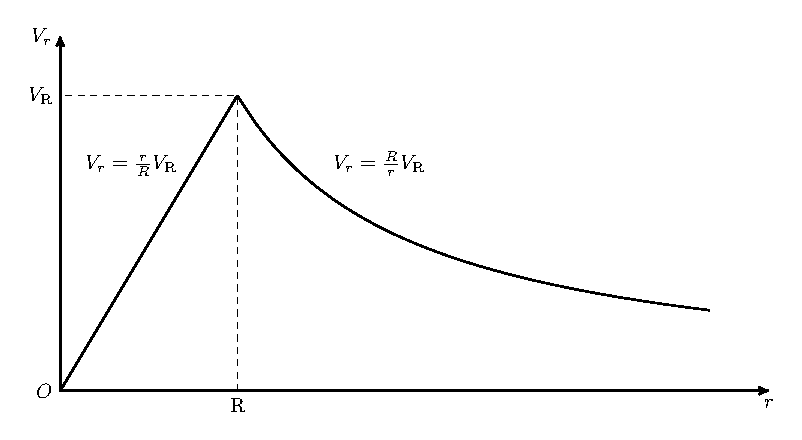
\includegraphics[width=0.6\textwidth]{Rankine.pdf}
  \caption{Rankine涡模型中切向速度沿涡半径的变化曲线图}
  \label{fig:Rankine}
\end{figure}



\section{龙卷风的数值模拟}
本文选择Ward型龙卷风发生装置(Ward-type Tornado Vortex Chamber,下文简称Ward-TVC)\cite{ward1972exploration}的改进版(Purdue-TVC)\cite{church1979characteristics}进行数值模拟,Purdue-TVC的示意图见图\ref{fig:Ward-TVC}。
Davies-Jones\cite{davies1976laboratory}详细评述了各种龙卷风发生装置,认为Ward-TVC与实际发生的龙卷风之间具有较好的几何和动力学相似性(geometric and dynamic similarity)。

控制龙卷风风场的主要无量纲参数为\cite{lewellen1993tornado}:
高宽比$A$、涡流比$S$、雷诺数(Reynolds number)$\mathrm{Re}$、弗劳德数(Froude number)$\mathrm{Fr}=\left( \Delta P/ 2g\Delta \rho z\right)^{1/2}$;$\Delta P$为气压降、$\Delta \rho$为流域内空气密度的变化、$g$为重力加速度、$z$为距离地面的高度。
高宽比和涡流比的定义如下:
\begin{equation}
  A = H_0/R_0
\end{equation}
\begin{equation}
  S = V_t/2A V_r
\end{equation}
其中$R_0$为上升气流孔的半径,$H_0$为气流入口的高度(见图\ref{fig:Ward-TVC}),
$V_t$和$V_r$为$R_0$处的切向和径向入流速度。
试验\cite{ward1972exploration}\cite{church1979characteristics}\cite{snow1982review}和数值模拟\cite{davies1976laboratory}等说明涡流比是控制龙卷风风场特征的最主要参数。
图\ref{fig:swirl}展示了龙卷风风场结构随涡流比的增大而发生变化\cite{hangan2008swirl}。
\begin{figure}[!htbp]
  \centering
  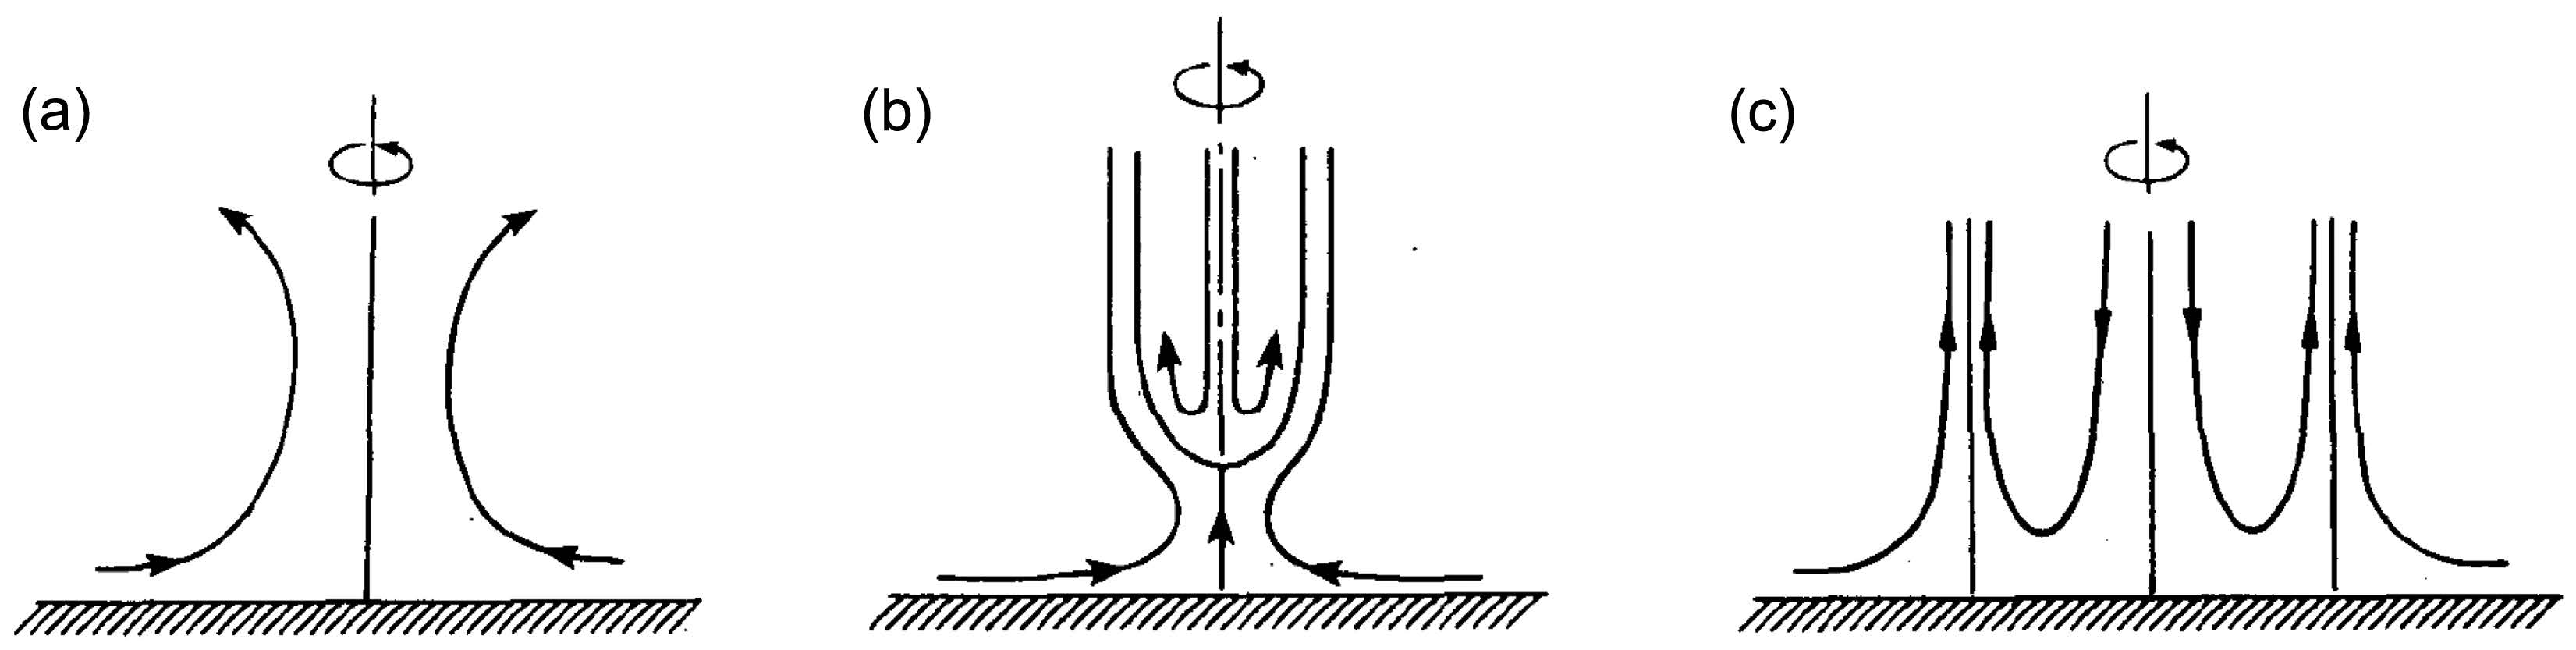
\includegraphics[width=\textwidth]{swirl_ratio_tornado_flow_pattern.jpg}
  \caption{增大涡流比引起龙卷风风场结构发生变化的示意图}\label{fig:swirl}
\end{figure}

随着涡流比的增大,龙卷风从射流状流场变化为单涡状涡旋(图\ref{fig:swirl}(a)),接着风场产生一个驻点、涡旋脱离地面(图\ref{fig:swirl}(b)),最后涡旋着地,分裂形成双涡状龙卷风(图\ref{fig:swirl}(c))。

本节主要介绍计算流体力学软件ANSYS Fluent模拟Ward-TVC的方法,并探讨涡流比对数值风场的影响。

\subsection{风场几何区域}
数值模拟的计算流域取Purdue-TVC的阴影区域,见图\ref{fig:Ward-TVC}。
为了与Baker\cite{baker1981boundary}的试验进行对比以验证数值风场的正确性,
取计算流域的尺寸及边界条件如图\ref{fig:tornado-domain}所示。
其中$X$轴对应龙卷风风场的径向,$Z$轴对应龙卷风风场的竖向。
\begin{figure}[!htbp]
  \begin{subfigure}[b]{0.5\textwidth}
    \centering
    \input{figures/tornado/Ward_TVC_sketch.pdf_tex}
    \caption{Purdue-TVC龙卷风发生装置示意图}\label{fig:Ward-TVC}
  \end{subfigure}
  \begin{subfigure}[b]{0.5\textwidth}
    \centering
    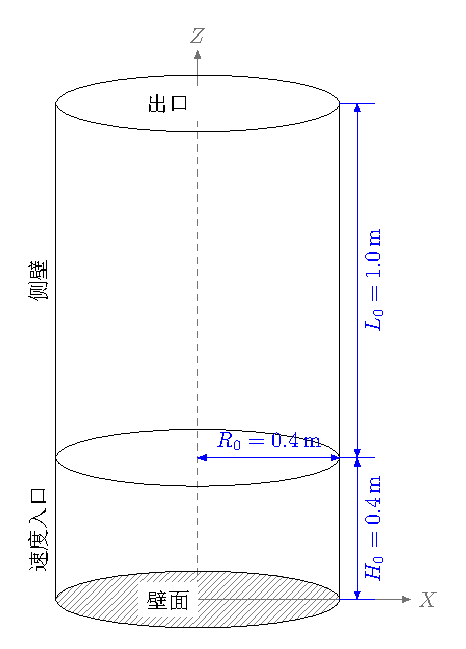
\includegraphics{domain.pdf}
    \caption{龙卷风数值模型的计算流域}\label{fig:tornado-domain}
  \end{subfigure}
  \caption{龙卷风发生装置和计算流域示意图}\label{fig:TVC-domain}
\end{figure}


\subsection{网格划分}
采用适应性良好的六面体结构化网格进行计算流域的划分。
初始网格数量大概为$300,000$,然后根据速度梯度和Y+进行自适应网格划分\cite{fluent2015user}。由于工程实际主要关注近地面附近龙卷风对结构的作用,
故细分主要针对近地面流域处的网格。不断加密网格直到近地面最大切向速度和最大切向速度所在半径的位置前后两次计算结果相差小于$5\%$。最后根据计算机的能力及计算结果的有效性,采用的网格数量为$1,536,000$。


\subsection{湍流模型}
龙卷风风场是旋流流场,根据Launder\cite{launder1989second}的研究,采用雷诺应力方程模型 (RSM)较为合适。
模型参数为:$C_{\mu}=0.09$; $C_{1\varepsilon}=1.44$; $C_{2\varepsilon}=1.92$; 
$C1-ps=1.8$; $C2-ps=0.6$; $C1'-ps=0.5$; $C2'-ps=0.3$。
湍流动能(TKE)普朗特数为 $1$; 湍动耗散率(TDR)普朗特数为 $1.3$。

\subsection{边界条件}
速度入口处径向和切向速度分布采用如下形式:
\begin{equation}\label{eqn:Vr}
  V_r(z) = V_0 \times (z/z_0)^{1/7}
\end{equation}
\begin{equation}\label{eqn:Vt}
  V_t(z) = 2 \times S \times V_r(z)
\end{equation}
式中,$V_r$为径向速度,$V_t$为切向速度,$V_0$为参考速度,$z_0$为参考高度,$S$为涡流比。

图\ref{fig:bc-inlet}为公式\eqref{eqn:Vr}和\eqref{eqn:Vt}所定义的风速分布与Baker\cite{baker1981boundary}试验的对比。
注意到试验风速分布与试验装置有关,而非实际的大气边界层风速分布。
公式\eqref{eqn:Vr}和\eqref{eqn:Vt}类似于大气边界层风速分布,并尽可能与Baker\cite{baker1981boundary}试验保持一致。
\begin{figure}[!htbp]
  \centering
  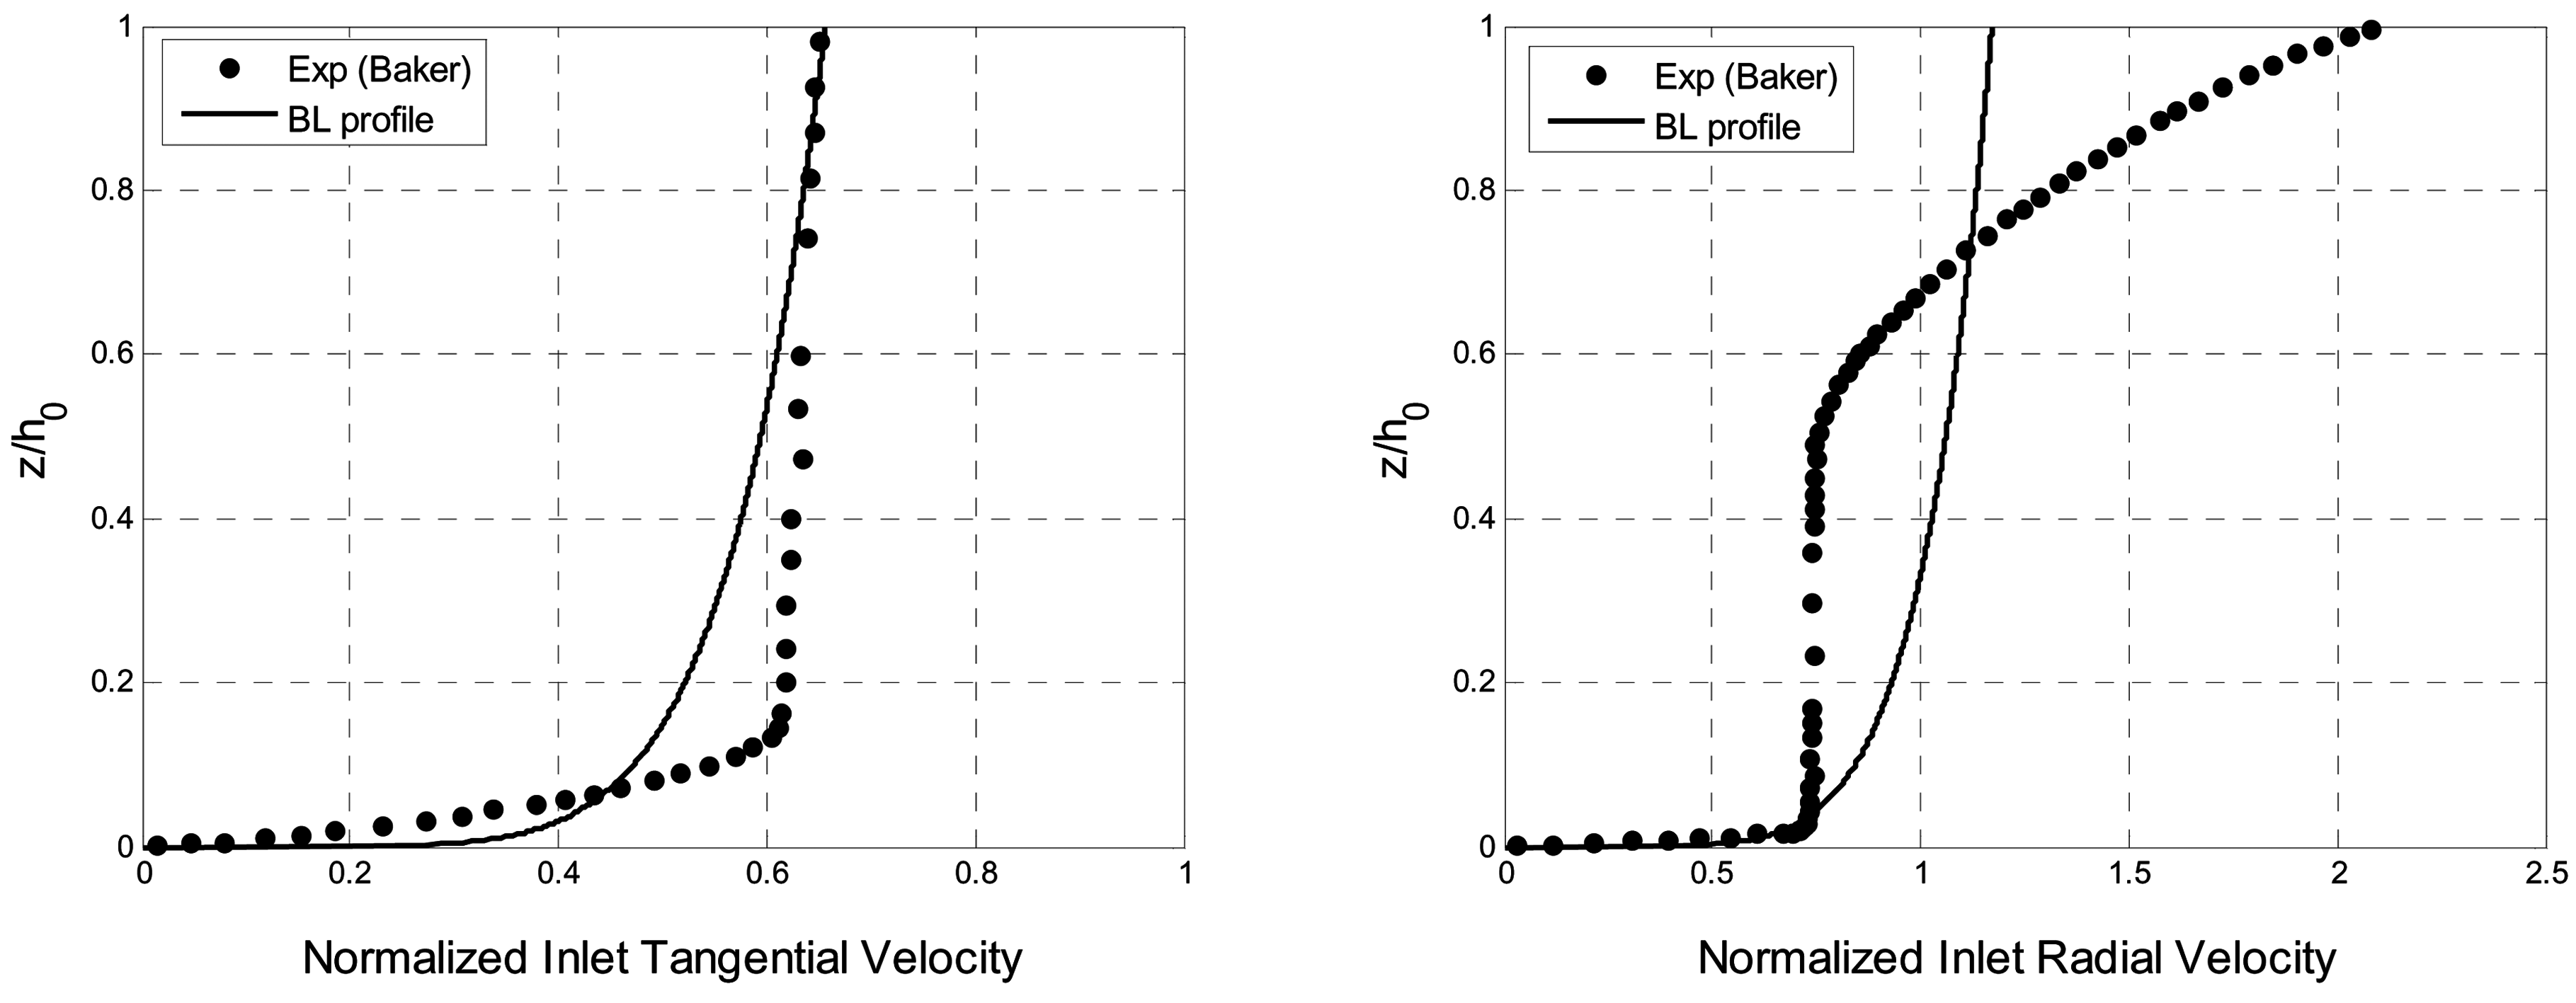
\includegraphics[width=\textwidth]{bc_inlet.png}
  \caption{入口处规格化切向和径向速度与Baker\cite{baker1981boundary}试验的对比}
  \label{fig:bc-inlet}
\end{figure}

试验表明,沿壁面法线方向的不同距离,可以将近壁面区域分成三层区域。
最里层,又称粘性底层,流动区域很薄,粘性力在动量、热量及质量交换中都起主导作用;
最外层为对数率层,粘性力不起主要作用;
两层之间的区域为过渡层,粘性力作用与湍流作用相当。

为描述粘性底层和对数率层内的流动,现引入无量纲参数$u^{+}$和$y^{+}$:
\begin{equation}
  u^{+} = \frac{u}{u_{\tau}}
\end{equation}
\begin{equation}
  y^{+} = \frac{y u_{\tau}}{\nu} = \frac{y}{\nu} \sqrt{\frac{\tau_w}{\rho}}
\end{equation}
式中:$u$是流体的时均速度、$u_{\tau}=\sqrt{\tau_w/\rho}$为壁面摩擦速度、$\tau_w$为壁面处切应力、$\nu$为空气动粘度系数、$y$为壁面第一层节点到壁面的距离。

以$y^{+}$的对数为横坐标,以$u^{+}$为纵坐标,可将壁面区域内的三个区域表示为图\ref{fig:uplus}所示\cite{fluent2015theory}。
\begin{figure}[!htbp]
  \centering
  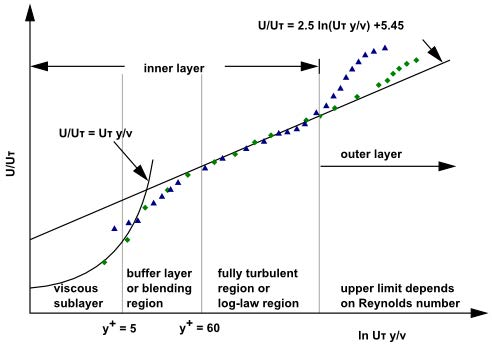
\includegraphics[width=0.6\textwidth]{figures/tornado/uplus.jpg}
  \caption{近壁面区域划分}\label{fig:uplus}
\end{figure}

通常有两种方法模拟近壁面区域:
一种采用“壁面方程”的半经验公式模拟受粘性力影响较大的区域,能够较好地修正湍流模型,解决壁面的存在对流场的影响;
另一种方法采用低$\mathrm{Re}$数的$k-\varepsilon$模型来求解粘性底层和过渡层,越靠近壁面,网格划分就越细,这种方法被称为“近壁面模型”法。
图\ref{fig:wall-treatment}为两种方法的对比\cite{fluent2015theory}。
\begin{figure}[!htbp]
  \centering
  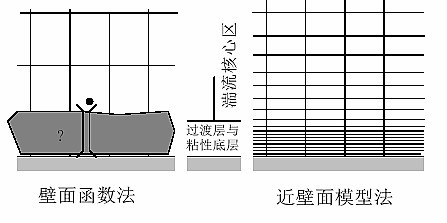
\includegraphics[width=0.8\textwidth]{wall_treatment.jpg}
  \caption{近壁面区域处理方法}
  \label{fig:wall-treatment}
\end{figure}

本文地面处采用强化壁面函数(Enhanced wall treatment\cite{fluent2015user}),需要对近壁面的网格进行细化。
边界层网格节点是否合适需要检查计算后的$y^{+}$值。
$y^{+}=u_{\tau} y/\nu$小于$1.5$能取得较好效果。

Smith的数值模拟\cite{smith1987effect}说明了侧壁的边界条件的选取对汇集区风场(主要关注的区域)的影响很小。
因此选择无滑壁面条件。

Purdue-TVC出口处设置了蜂窝板,能使气流竖直流出,还能阻止排风机对涡旋的影响。
试验中排风机驱动了流场运动,而在数值模型中,入口风速驱动了流场运动,且不包含排风机的影响,因此数值模型出口处不需设置代表直流蜂窝板的边界条件。根据Smith\cite{smith1987effect}的论述,上边界更合适的边界条件为压强出口边界条件(pressure-outflow)。
此边界条件假设除压强外的所有物理量在边界的法向梯度为零\cite{fluent2015user}。



\subsection{控制方程及求解选项}
控制方程采用非定常雷诺平均纳维-斯托克斯方程(Unsteady Reynolds Averaged Navier-Stokes, RANS)。
时间离散采用一阶隐性格式,压强速度场的耦合采用压力修正的分离式算法,SIMPLEC算法。
动量、TKE、TDR和雷诺应力采用二阶迎风格式。



\section{数值模拟结果及其正确性验证}\label{sec:tornado}
图\ref{fig:tornado-domain}所示的风场几何区域,建立柱面坐标系$\{O:r \theta z\}$。
本文主要关注在柱面坐标系下数值风场的速度特征,其中径向(radial)、切向(tangential)、竖向(axial)风速分别记为$V_r(r,\theta,z)$、$V_t(r,\theta,z)$和$V_a(r,\theta,z)$。

考虑到龙卷风风场具有轴对称性,故对数值风场速度分布沿圆周($r=$常数)进行平均,消除速度随$\theta$的变化,得到轴对称的风场$V_r(r,z)$、$V_t(r,z)$和$V_a(r,z)$。

将上述轴对称风场与Baker试验\cite{baker1981boundary}结果及多普勒雷达实测风场进行对比,以验证数值风场的正确性。
并探讨缩尺龙卷风数值风场转化为足尺风场的方法。



\subsection{Baker试验对比}
Baker利用Purdue-TVC进行了龙卷风风场的试验模拟\cite{baker1981boundary},选取$S=0.28$的风场在$r/R_0=0.1025$和$r/R_0=0.2125$处风速各分量随高度变化曲线与数值风场进行对比。
将高度以$R_0$进行无量纲化,速度以入口平均径向速度$U_0=Q/(R_0 H_0)$进行无量纲化,其中$2\pi Q$为速度入口边界处的流量。
将\eqref{eqn:Vr}定义的速度入口边界的径向速度代入可得:
\begin{equation}
  U_0 = \frac{Q}{R_0 H_0} = \frac{R_0 \int_0^{H_0} V_r(z)\,\mathrm{d}z}{R_0 H_0} = \frac{\int_0^{H_0} V_0 (z/z_0)^{1/7}\,\mathrm{d}z}{H_0} = \frac{7}{8} V_0 \left(\frac{H_0}{z_0}\right)^{1/7}
\end{equation}

图\ref{fig:cfd_vs_exp_Vr}、图\ref{fig:cfd_vs_exp_Vt}和图\ref{fig:cfd_vs_exp_Va}分别为数值风场(CFD)与Baker试验无量纲化径向、切向和轴向风速随高度变化的对比图。
二者总体上吻合较好。

\begin{figure}[!htbp]
  \centering
  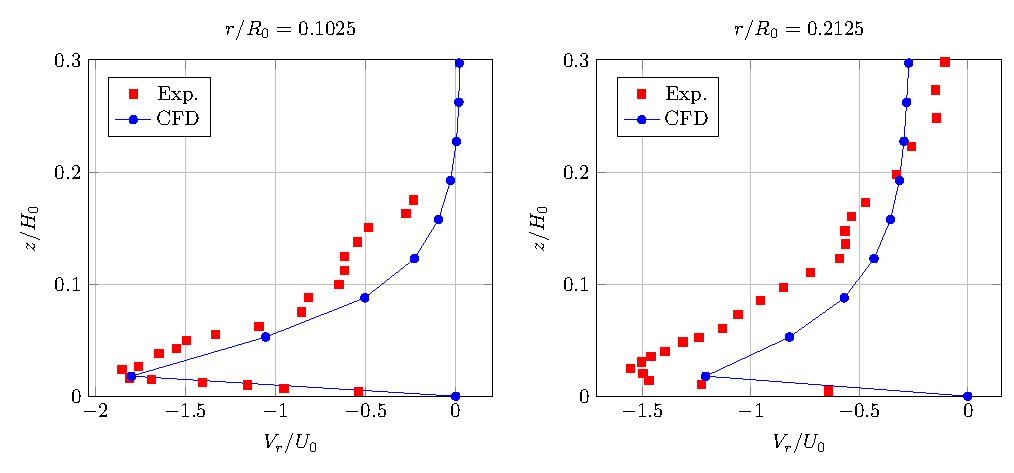
\includegraphics[width=1.0\textwidth]{cfd_vs_exp_Vr.pdf}
  \caption{数值风场与Baker试验无量纲化径向速度随高度变化的对比,$S=0.28$}
  \label{fig:cfd_vs_exp_Vr}
\end{figure}
\begin{figure}[!htbp]
  \centering
  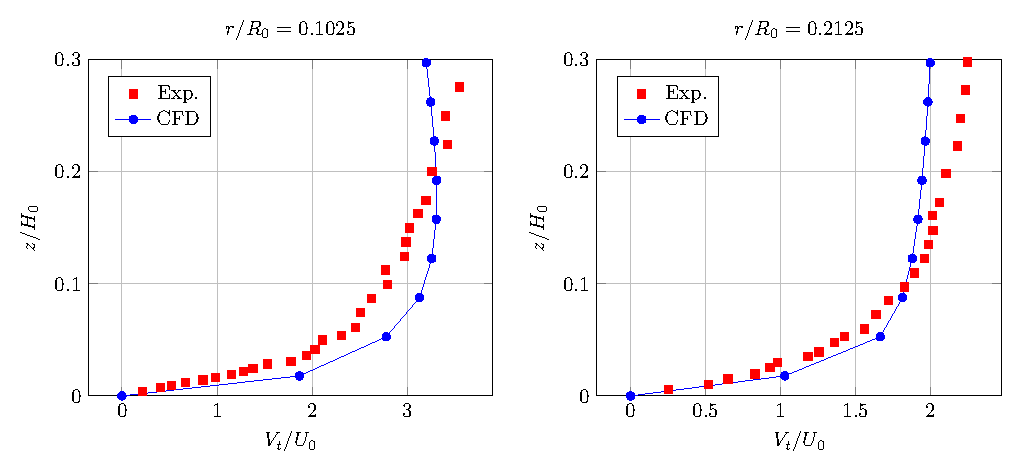
\includegraphics[width=1.0\textwidth]{cfd_vs_exp_Vt.pdf}
  \caption{数值风场与Baker试验无量纲化切向速度随高度变化的对比,$S=0.28$}
  \label{fig:cfd_vs_exp_Vt}
\end{figure}
\begin{figure}[!htbp]
  \centering
  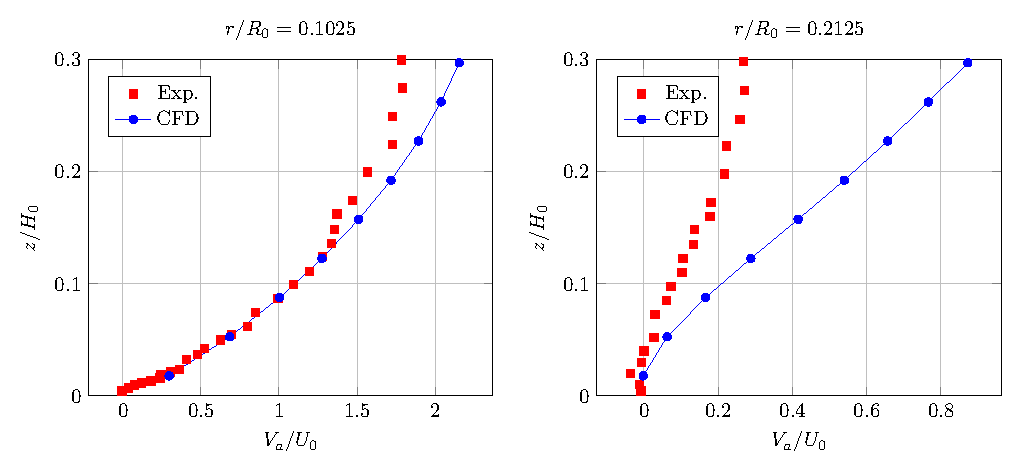
\includegraphics[width=1.0\textwidth]{cfd_vs_exp_Va.pdf}
  \caption{数值风场与Baker试验无量纲化竖向速度随高度变化的对比,$S=0.28$}
  \label{fig:cfd_vs_exp_Va}
\end{figure}

\subsection{数值风场的风速分布特征}
图\ref{fig:Vt-x=0}为计算流域轴向剖面($X=0$)处切向速度云图。
从图中可以明显看出涡旋中心处切向速度接近于零;
图\ref{fig:Vt-z=30mm}为\SI{30}{mm}高度处的切向速度云图,可以看出流域的涡旋接近中心轴线,并能显示出漏斗状形态,显示了龙卷风风场具有很好的涡旋特性。
由图\ref{fig:Vt}可知龙卷风涡旋中心的切向速度较小,在核心半径处达到最大,而后随着远离涡旋中心的距离增大而逐渐减小。
且在核心半径内,切向速度的变化较快,而远离核心半径时,变化逐渐缓和,与Rankine模型吻合较好。
此外还可看出随着离地高度的增加,核心半径有所增大,而最大切向风速呈逐渐减小的趋势。
\begin{figure}[!htbp]
  \begin{subfigure}[b]{0.5\textwidth}
    \centering
    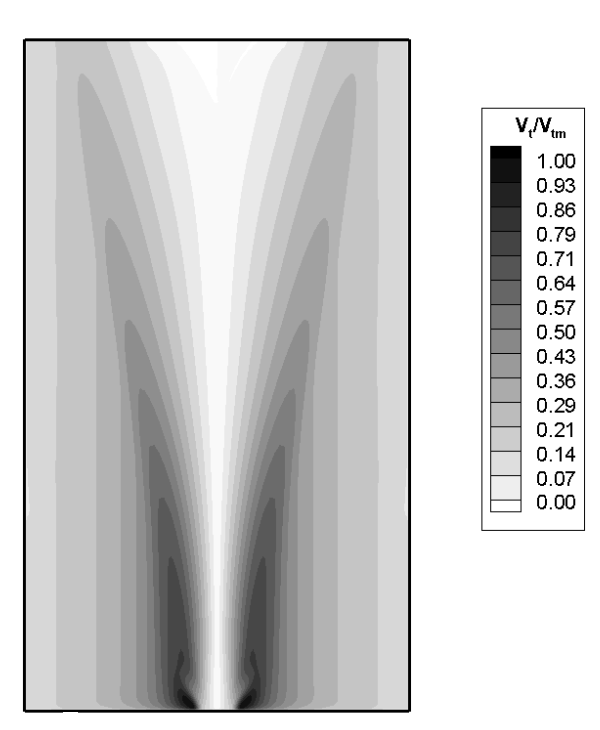
\includegraphics[width=\textwidth]{Vt_x=0.png}
    \caption{轴向剖面($X=0$)}\label{fig:Vt-x=0}
  \end{subfigure}
  \begin{subfigure}[b]{0.5\textwidth}
    \centering
    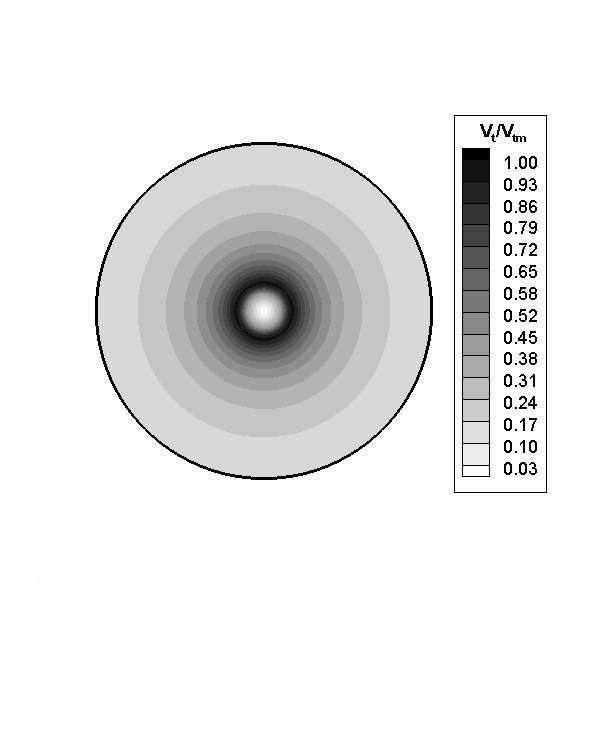
\includegraphics[width=\textwidth]{Vt_z=30mm.png}
    \caption{水平剖面($Z=\SI{30}{mm}$)}\label{fig:Vt-z=30mm}
  \end{subfigure}
  \caption{切向速度云图}\label{fig:Vt-contour}
\end{figure}

\begin{figure}
  \centering
  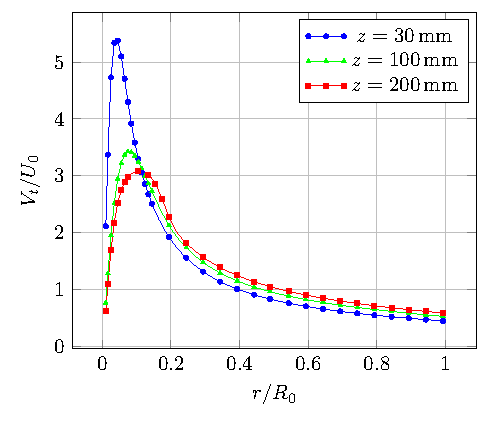
\includegraphics[width=0.6\textwidth]{Vt.pdf}
  \caption{数值风场不同高度处切向速度沿径向的变化图,$S=0.28$}
  \label{fig:Vt}
\end{figure}

\subsection{数值风场的风压分布特征}
图\ref{fig:P-x=0}和图\ref{fig:P-z=30mm}分别给出了计算流域轴向剖面($X=0$)和水平剖面($Z=\SI{30}{mm}$)处风压云图,$P_m$是风场最大静压,为负压。
可以看出龙卷风中心处离地面一定高度范围内存在很强的负压,且随着半径的增加而逐渐减小。

图\ref{fig:p}给出了三种不同高度处的风压沿径向的分布,可以看出不同高度处风压分布接近一致。

\begin{figure}[!htbp]
  \begin{subfigure}[b]{0.5\textwidth}
    \centering
    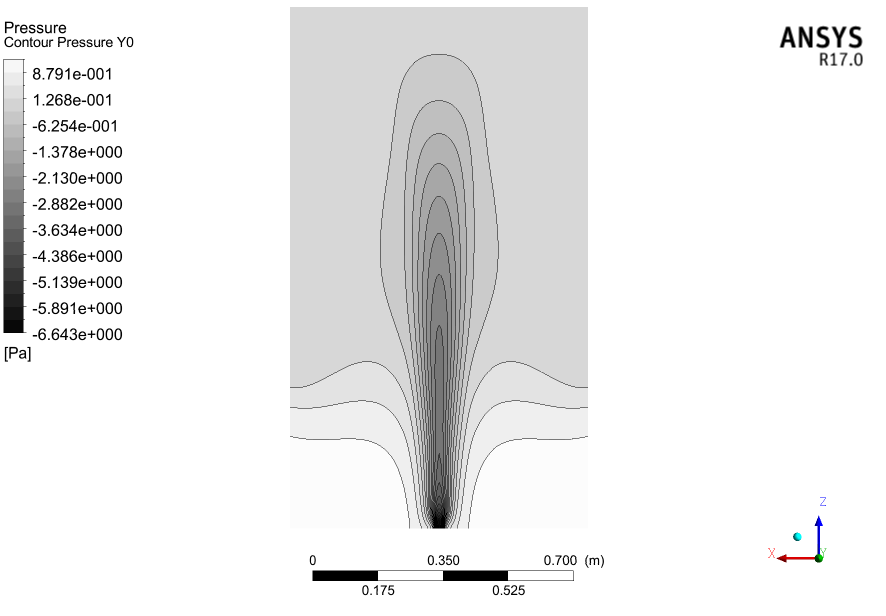
\includegraphics[width=\textwidth]{P_x=0.png}
    \caption{轴向剖面($X=0$)}\label{fig:P-x=0}
  \end{subfigure}
  \begin{subfigure}[b]{0.5\textwidth}
    \centering
    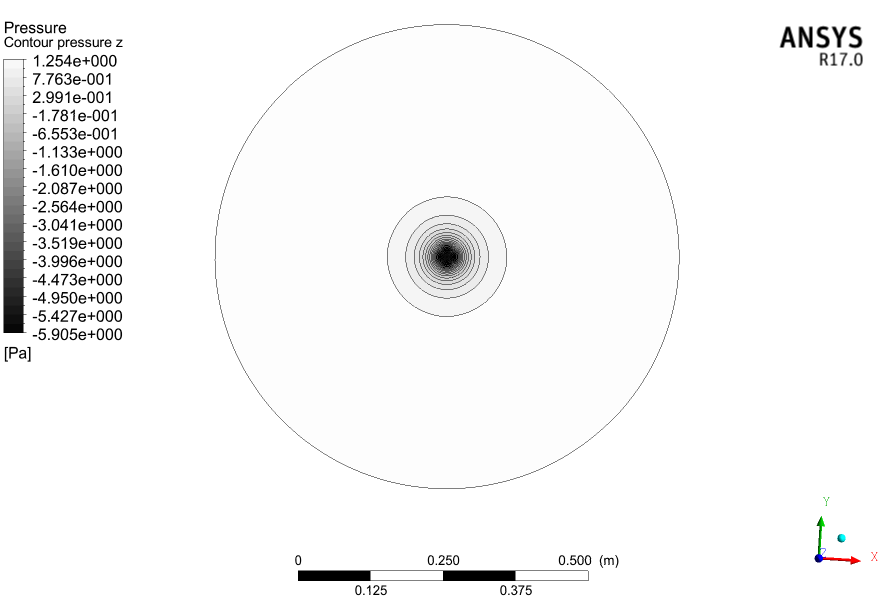
\includegraphics[width=\textwidth]{P_z=30mm.png}
    \caption{水平剖面($Z=\SI{30}{mm}$)}\label{fig:P-z=30mm}
  \end{subfigure}
  \caption{风压云图}\label{fig:p-contour}
\end{figure}

\begin{figure}[!htbp]
  \centering
  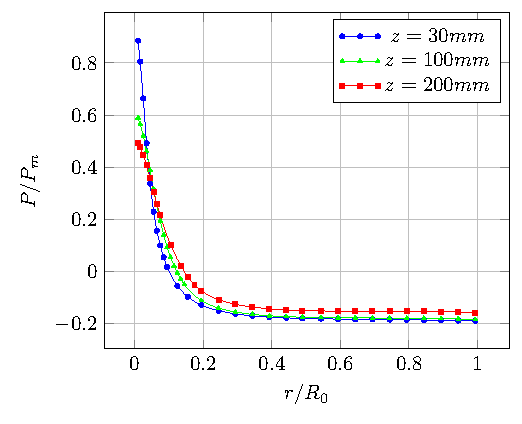
\includegraphics[width=0.6\textwidth]{p.pdf}
  \caption{数值风场不同高度处风压沿径向的变化图}
  \label{fig:p}
\end{figure}

\subsection{实测龙卷风风场对比}
为了进一步验证数值龙卷风风场的有效性,选用1998年5月发生在美国南达科他州Spencer地区的实测龙卷风风场进行对比。
这些数据由车载式多普勒雷达采集,Wurman等人有详细的介绍\cite{wurman2002multiple}\cite{alexander2005spencer}\cite{wurman2005spencer}。

采集的风场在不同竖向高度处、\SI{2}{km}$\times$\SI{2}{km}的水平区域内(水平测点间距为\SI{20}{m})。
将原始风场去除龙卷风平移速度,得到涡旋风场,并利用最小二乘原理将速度场沿圆周平均,以消除多涡等因素的影响。
最终得到的龙卷风切向速度随离开涡旋中心径向距离的变化关系如图\ref{fig:Vt-full}所示。
\begin{figure}[!htbp]
  \centering
  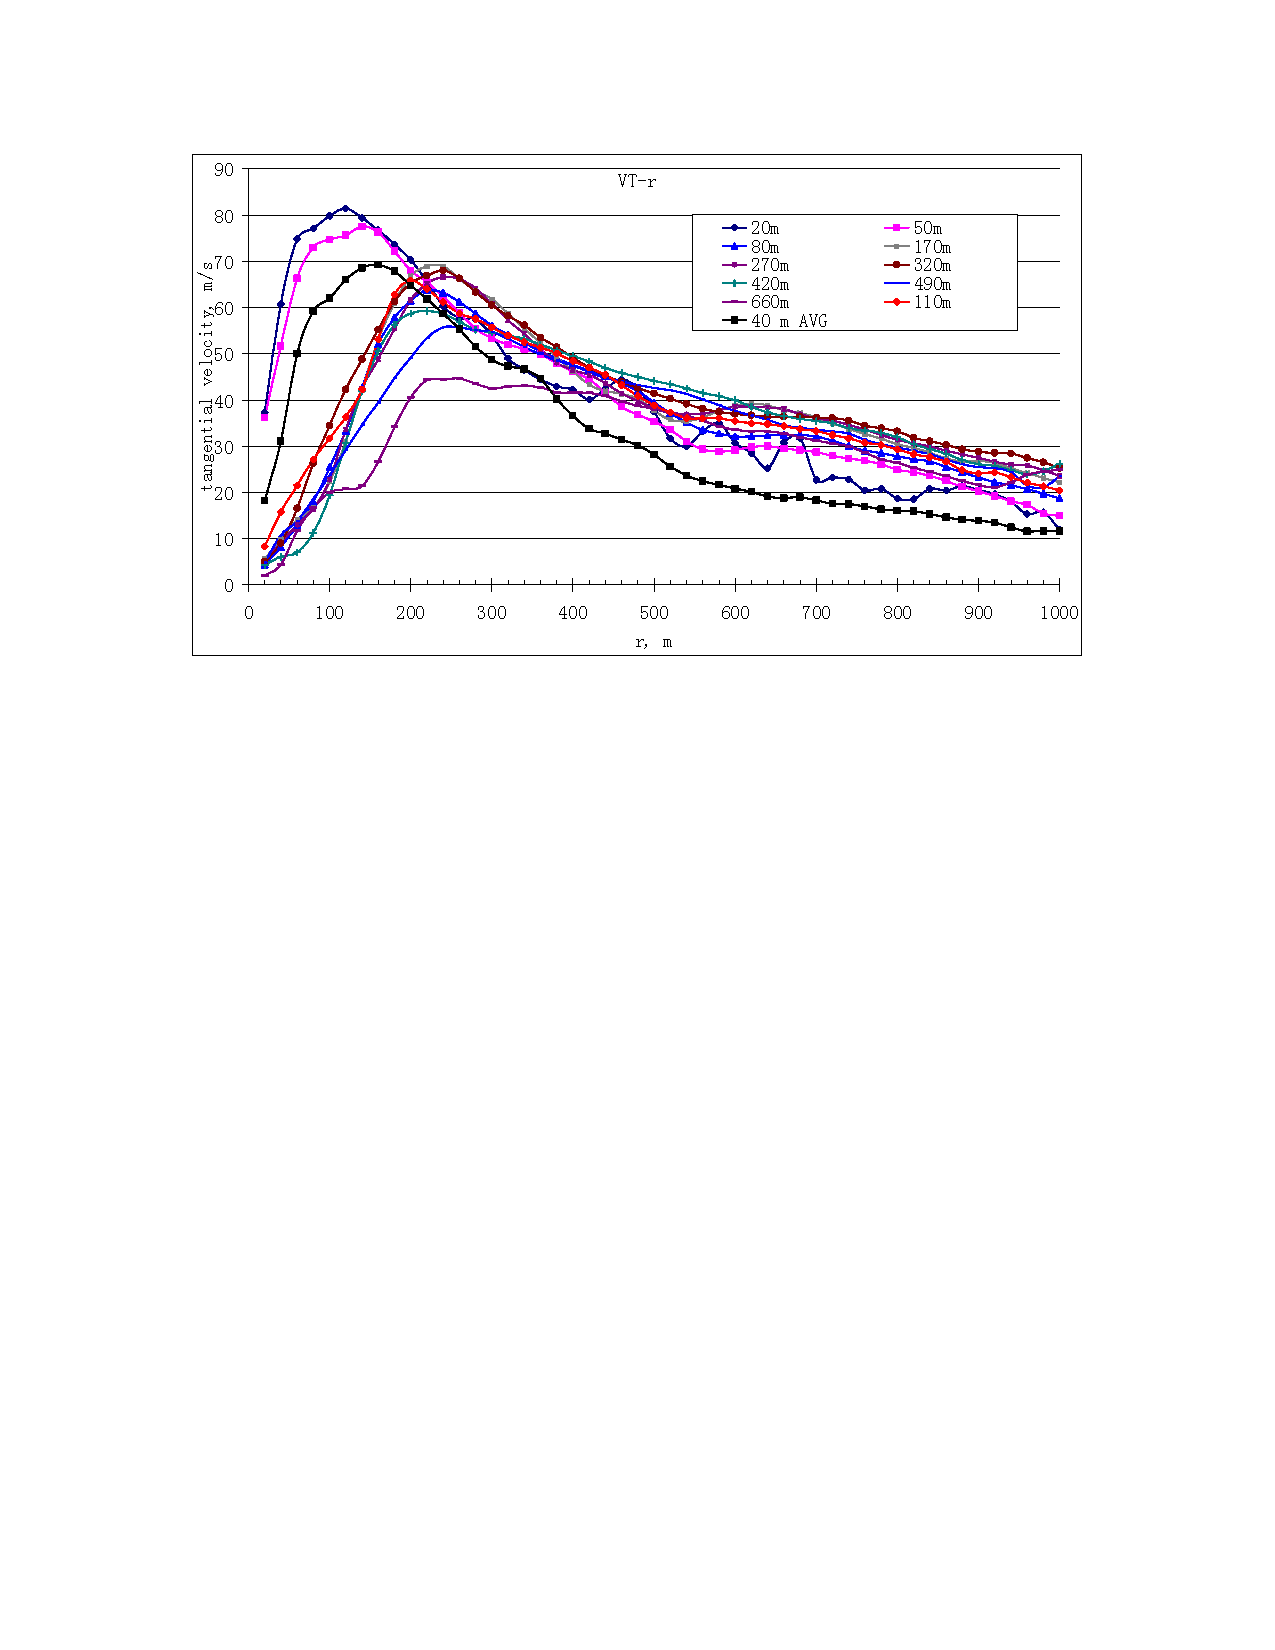
\includegraphics[width=0.8\textwidth]{Vt_full.pdf}
  \caption{实测风场在不同高度处切向速度与径向距离的关系曲线\cite{sarkar2005velocity}}
  \label{fig:Vt-full}
\end{figure}

% \graphicspath{{figures/tower/}}
\chapter{输电塔结构有限元建模}\label{chapter:tower}
\section{\SI{500}{kV}南京三江口长江大跨越工程介绍}
\SI{500}{kV}南京三江口长江大跨越工程是山西阳城电厂二期工程电力送出江苏省
内配套等输变电工程的重要组成部分,跨越点在长江南京河段的三江口节点位置。
按耐—直—直—耐实施跨越,档距分布为\SI{520}{m}-\SI{1770}{m}-\SI{520}{m}(图\ref{fig:tower-line}),跨越塔与跨越塔之间的输电线矢高为\SI{132.4}{m},跨越塔与锚塔之间的输电线矢高为\SI{50}{m}。
\begin{figure}[!htbp]
\centering
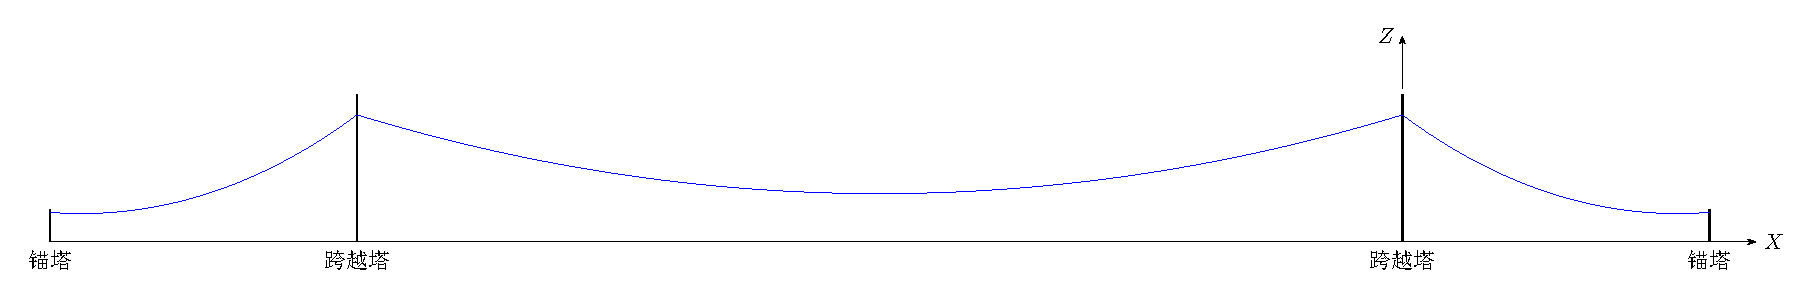
\includegraphics[width=\textwidth]{tower_line_system.pdf}
\caption{三江口大跨越示意图}
\label{fig:tower-line}
\end{figure}

大跨越南、北跨越塔均为双回路蝶型布置的钢管塔,呼高\SI{215}{m},全高\SI{249.5}{m},根开\SI{49.6}{m},单基塔重(含旋梯及走道)共\SI{1924}{t}。
钢管塔最大管径\SI{1480}{mm},相应壁厚\SI{25}{mm},钢管材质采用Q345B和Q235B级钢,最大螺栓直径\SI{56}{mm},螺栓采用6.8级和8.8级两种。
大跨越输电塔(下文简称大跨越塔)实物如图\ref{fig:real-tower}所示。
锚塔为单回干字型角钢塔,锚塔横担垂直于跨越段中心线布置,根开为\SI{16}{m}$\times$\SI{24}{m}布置,呼高\SI{24}{m},全高\SI{55}{m},单基塔重\SI{106}{t}。
每个回路分别对应2基铁塔,共使用4基锚塔。

导线采用四分裂布置,型号为 AACSR/EST-500 特强钢芯铝合金绞线,两根地线采用 36芯的OPGW-325型复合光缆,光缆为层绞结构。
导线、OPGW均为整根,跨越耐张段没有接头。锚塔上跳线采用LGJ-630/45型钢芯铝绞线,越侧耐张绝缘子串引流线夹与LGJ-630/45型钢芯铝绞线匹配。跨越塔导线采用四联530k N级盘瓷悬垂绝缘子串,OPGW采用双联预绞式悬垂金具串;锚塔导线采用六联400k N级盘瓷耐张绝缘子串,OPGW采用预绞式耐张金具串。
\begin{figure}[!htbp]
\centering
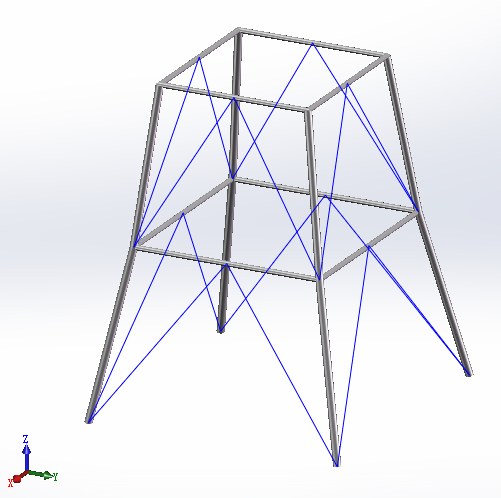
\includegraphics[width=\textwidth]{tower.png}
\caption{三江口大跨越输电塔}
\label{fig:real-tower}
\end{figure}

\section{输电塔有限元模型}
本文选择大型通用有限元软件ANSYS Mechanical APDL进行输电塔建模。

\subsection{输电塔塔体模拟}\label{sec:tower-fea}
选用二节点非线性三维梁单元BEAM 188模拟输电塔构件。
单元每个节点处包括三个平动自由度和三个转动自由度。
输电塔构件之间为多孔螺栓连接,有限元模型以刚性节点模拟。
输电塔的有限元模型见\ref{fig:tower-fea}所示。
考虑到输电塔为空间对称结构,取塔的底面中心为坐标原点,高度方向为$Z$轴方向,输电线方向为$X$轴方向(图\ref{fig:tower-line}、\ref{fig:tower-fea})。
\begin{figure}[!htbp]
\centering
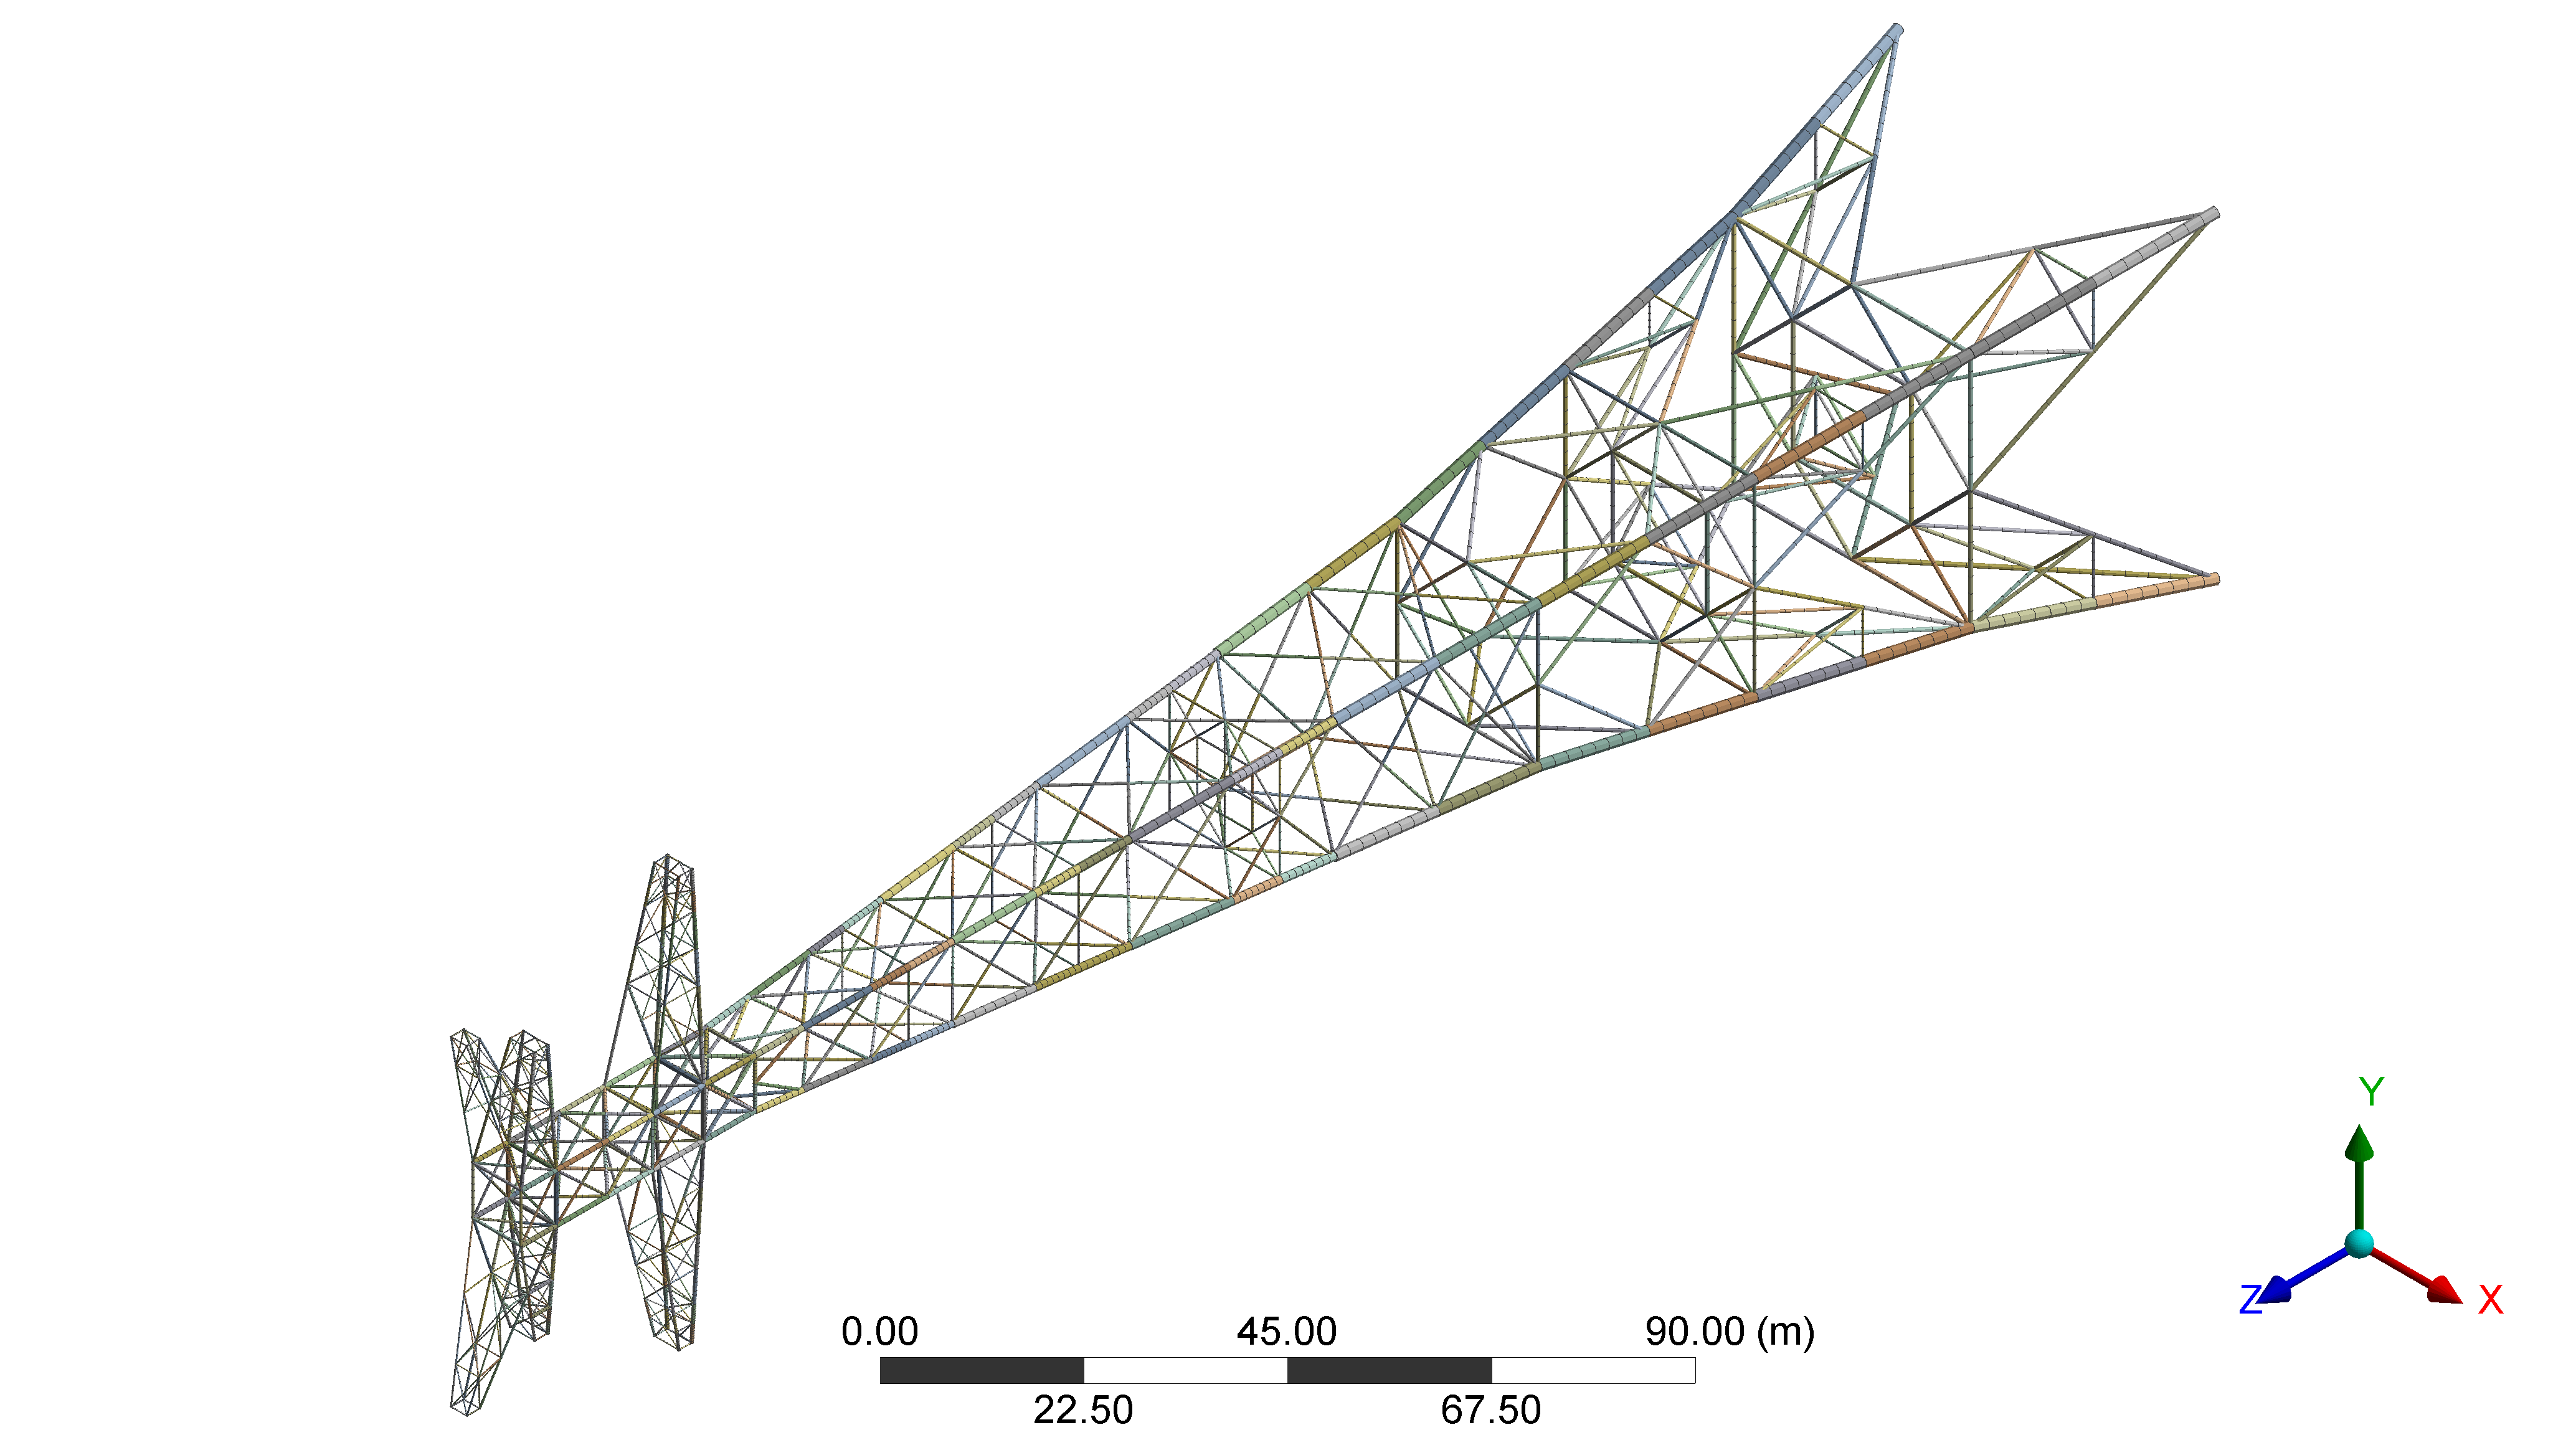
\includegraphics[width=\textwidth]{tower_fea.png}
\caption{输电塔有限元模型}
\label{fig:tower-fea}
\end{figure}

\subsection{输电导线模拟}


\section{输电塔结构模态分析}
本节对大跨越输电塔结构进行模态分析,计算其固有频率及振型,与文献对比,以验证输电塔有限元模型的正确性,并为后续的动态响应分析提供参考。

输电塔各阶固有频率及其与文献\cite{ren2010tower}的对比见表\ref{tab:freq},
各阶振型见图\ref{fig:modes}所示。

\begin{table}[!htbp]
  \centering
  \caption{输电塔固有频率$/\SI{}{Hz}$}
  \label{tab:freq}
  \begin{tabu} to 1.0\textwidth {X[1.5,c] X[1,c] X[1,c] X[1,c] X[1,c] X[1,c] X[1,c] X[1,c] X[1,c] X[1,c]}
  \toprule
  振型 & 1 & 2 & 3 & 4 & 5 & 6 & 7 & 8 & 9 \\
  \midrule
  频率\cite{ren2010tower} & 0.609 & 0.612 & 1.102 & 1.558 & 1.608 & 2.113 & 2.296 & 2.407 & 3.046 \\
  频率 & 0.613 & 0.615 & 1.093 & 1.565 & 1.594 & 2.084 & 2.312 & 2.363 & 2.368 \\
  \bottomrule
  \end{tabu}
\end{table}

\begin{figure}[!htbp]
  \centering
  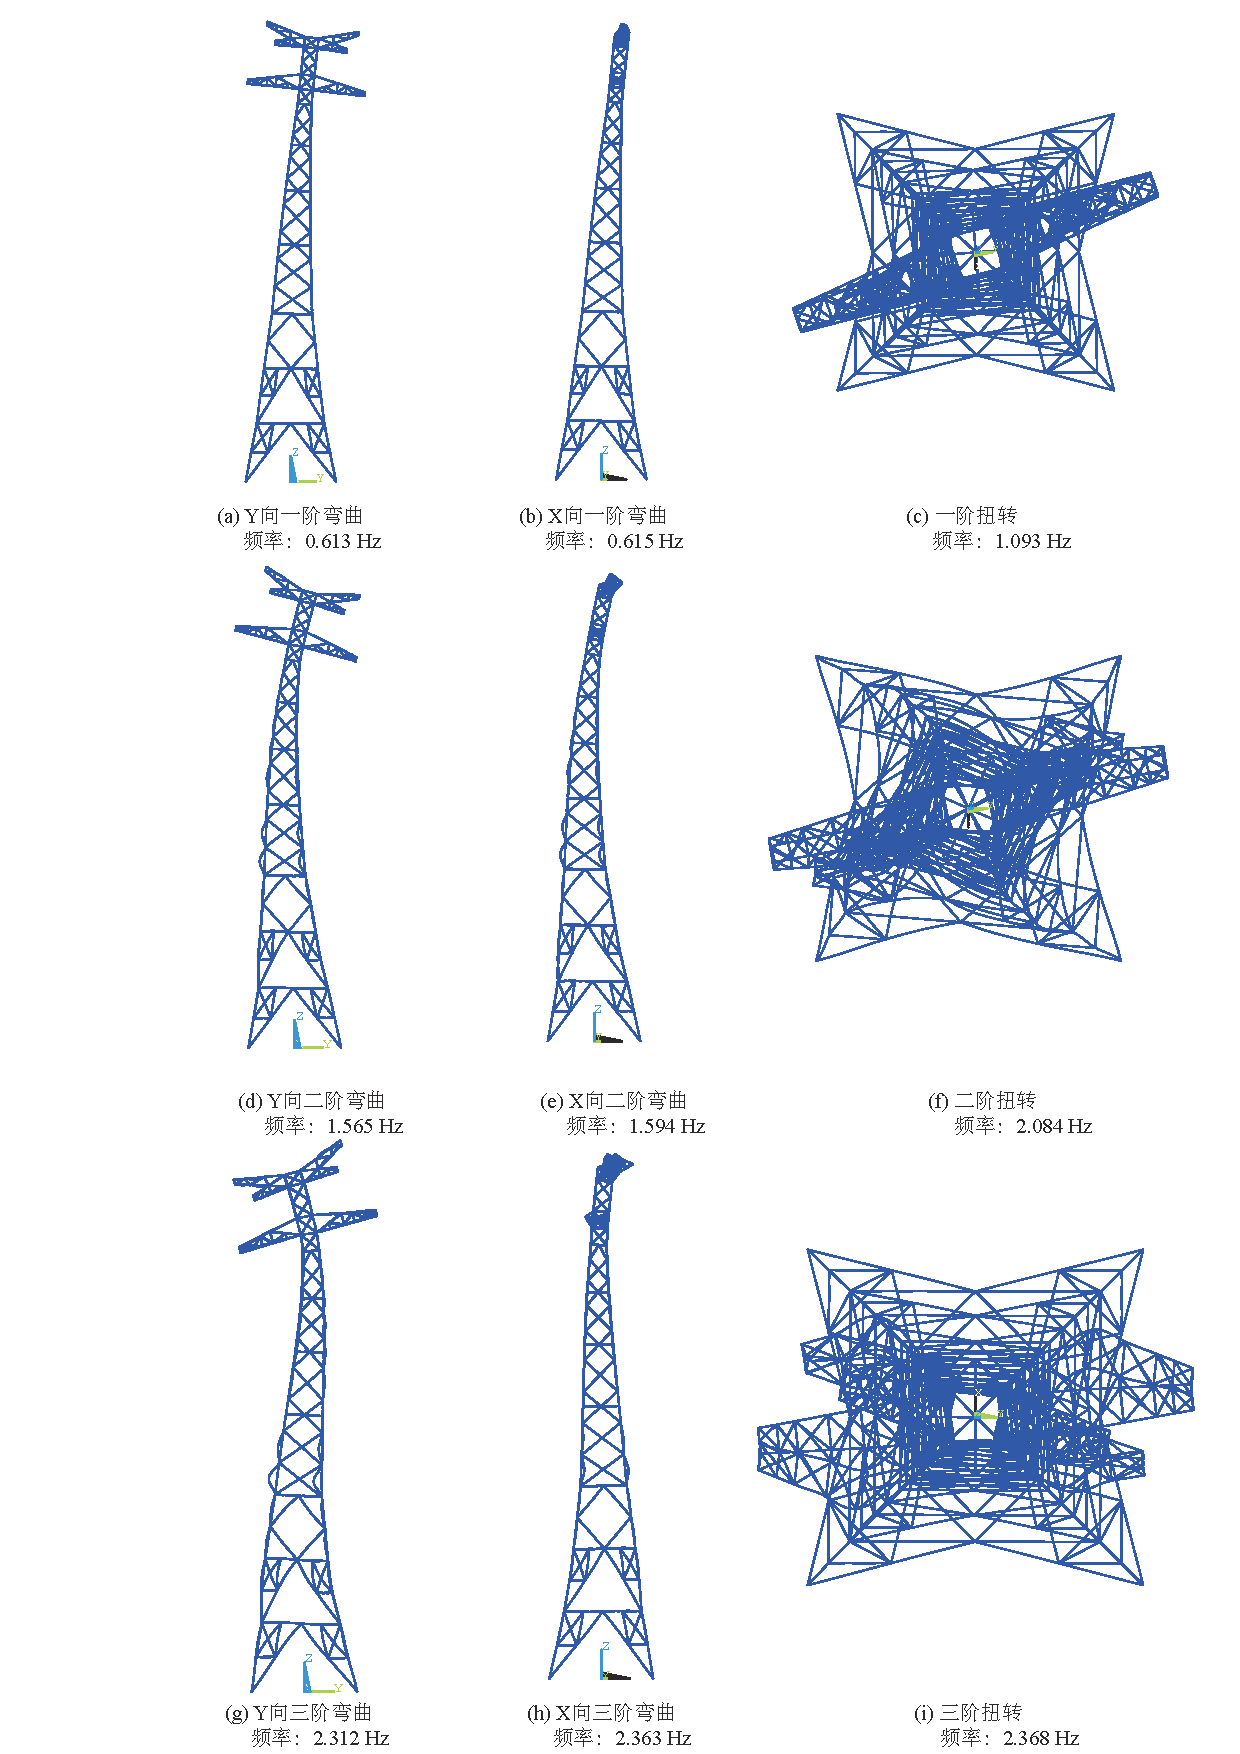
\includegraphics[width=0.9\textwidth]{modes.pdf}
  \caption{输电塔各阶振型图}
  \label{fig:modes}
\end{figure}

\graphicspath{{figures/static/}}
\chapter{输电塔结构在龙卷风作用下的静态响应分析}\label{chapter:static}

本章主要进行输电塔结构在龙卷风作用下的静态响应分析,即忽略龙卷风的平移效应,选定龙卷风核心相应于输电塔结构中心的位置,进行静力弹塑性分析。输电塔结构受到的主要荷载为:
\begin{enumerate}
\item 重力荷载
\item 输电塔受到的龙卷风涡旋风场的荷载
\item 输电线传到输电塔的荷载
\end{enumerate}
其中忽略了龙卷风对输电线的荷载,主要是因为:
\begin{enumerate}
\item 龙卷风路径宽度较小,F1-F2级龙卷风的路径宽度为\SI{60}{m}-\SI{150}{m}。
\item 输电线受到的风荷载作用机制比较复杂。
\end{enumerate}


\section{龙卷风风场处理}\label{sec:tornado}
输电塔在龙卷风风场中的水平投影示意图如图\ref{fig:tower-tornado-cs}所示。
\begin{figure}[!htpb]
  \centering
  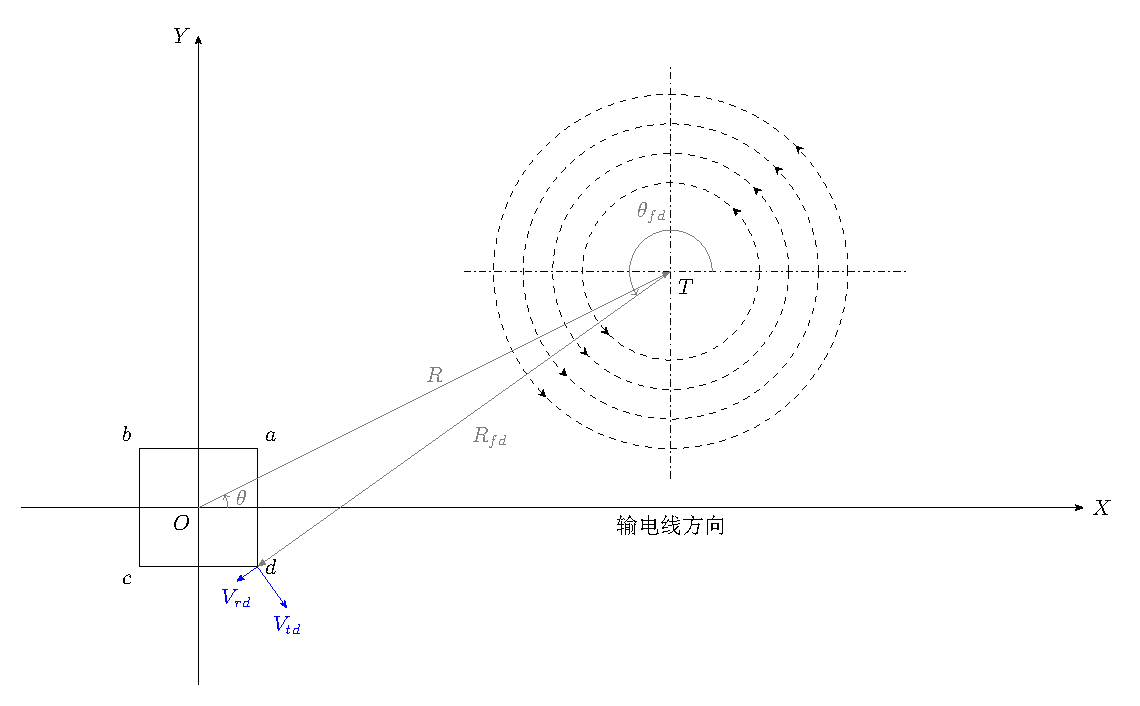
\includegraphics[width=\textwidth]{tower_tornado_cs.pdf}
  \caption{输电塔在龙卷风风场中的水平投影示意图}
  \label{fig:tower-tornado-cs}
\end{figure}
输电塔直角坐标系$\{O: XYZ\}$的建立方法见第\ref{sec:tower-fea}节。
$abcd$为输电塔处于同一水平剖面的节点。
下文主要展示推导$d$节点处龙卷风风速的方法,其余节点类似。
龙卷风中心在坐标系$\{O: XYZ\}$中的位置用极坐标$(R, \theta)$表示。
输电塔节点$d$相应于龙卷风核心的极坐标为$(R_{fd}, \theta_{fd})$,$d$节点受到的龙卷风切向、径向风速分别为$V_{td}$、$V_{rd}$,以及图\ref{fig:tower-tornado-cs}未明确表示的竖向风速$V_{ad}$。

\subsection{输电塔节点相应于龙卷风中心位置的极坐标}\label{sec:d-polor}
假设$d$节点在输电塔坐标系$\{O: XYZ\}$中的坐标为$(x_d, y_d, z_d)$,下文将推导节点$d$相应于龙卷风中心的极坐标$(R_{fd}, \theta_{fd})$。

龙卷风中心$T(R, \theta)$在输电塔坐标系$\{O: XYZ\}$中的直角坐标为$(R\cos\theta, R\sin\theta)$,则节点$d$相应于龙卷风中心$T$的向量为:
\begin{equation}
  \vv{Td} = \vv{Od} - \vv{OT} = (x_d - R\cos\theta, y_d - R\sin\theta) = R_{fd}(\cos\theta_{fd}, \sin\theta_{fd})
\end{equation}
式中,
\begin{equation}
\begin{split}
  R_{fd} & = \sqrt{(x_d-R\cos\theta)^2+(y_d-R\sin\theta)^2} \\
  \theta_{fd} & = \arctan \frac{y_d - R\sin\theta}{x_d - R\cos\theta}
\end{split}
\end{equation}

\subsection{龙卷风风场在直角坐标系下的分量}\label{sec:cs}
第\ref{sec:tornado}节模拟的龙卷风风场是定义在极坐标系下的,而施加风荷载采用直角坐标系下的风速分量较为简单,因此需要将龙卷风风场从极坐标系转化为直角坐标系。

输电塔节点$d$受到的龙卷风径向风速$V_{rd}$与$X$轴正方向的夹角为$\theta_{fd}$(图\ref{fig:tower-tornado-cs}),切向风速$V_{td}$与$X$轴正方向的夹角为$(\theta_{fd}+\pi/2)$,进行速度的分解如下:
\begin{equation}
\begin{split}
  V_{xd} & = V_{rd} \cos\theta_{fd} + V_{td} \cos(\theta_{fd}+\pi/2) \\
         & = V_{rd} \cos\theta_{fd} - V_{td} \sin(\theta_{fd}) \\
  V_{yd} & = V_{rd} \sin\theta_{fd} + V_{td} \sin(\theta_{fd}+\pi/2) \\
         & = V_{rd} \sin\theta_{fd} + V_{td} \cos(\theta_{fd}) \\   
  V_{zd} & = V_{ad}  
\end{split}
\end{equation}

有了上述准备工作,就可以计算输电塔上任意节点受到的龙卷风风速在直角坐标系下的分量了。

\subsection{龙卷风风场中任意节点处风速分量}
输电塔节点$d$相应于龙卷风中心的实际位置为$(R_{fd}, \theta_{fd})$(见第\ref{sec:d-polor}节),此节点对应于缩尺龙卷风风场$V_r(r,z)$、$V_t(r,z)$和$V_a(r,z)$(见第\ref{sec:tornado}节)中的位置为$(R_{md}, Z_{md})$,且
\begin{equation}
\begin{split}
  R_{md} & = R_{fd} / L_s \\
  Z_{md} & = z_{fd} / L_s
\end{split}
\end{equation}

在缩尺龙卷风风场中,由位置$(R_{md}, Z_{md})$可提取缩尺龙卷风风场径向、切向和竖向风速分量分别为$V_{rmd}$、$V_{tmd}$和$V_{amd}$。根据缩尺龙卷风速度相似比$V_s$可将其转化为足尺龙卷风风场中的速度分量:

\begin{equation}
\begin{split}
  V_{rd} &= V_{rmd} \times V_s \\
  V_{td} &= V_{tmd} \times V_s \\
  V_{ad} &= V_{amd} \times V_s
\end{split}
\end{equation}

最后根据第\ref{sec:cs}节的方法即可将输电塔节点$d$受到的极坐标系下的足尺龙卷风风速分量转化为直角坐标系下的风速分量。


\section{输电塔结构龙卷风风荷载计算}

\subsection{ASCE输电塔荷载规范风荷载计算方法}
ASCE主编的输电塔荷载规范 Guidelines for electrical transmission line structural loading\cite{wong2009guidelines}中输电塔风荷载计算公式为:
\begin{equation}
F = \gamma_{\mathrm{w}} Q K_{\mathrm{z}} K_{\mathrm{zt}} \left( V_{50}\right)^2 G C_{\mathrm{f}} A
\end{equation}
其中:
\begin{description}[leftmargin=!,labelwidth=2em]
\item[$F$] 顺风向风荷载
\item[$\gamma_{\mathrm{w}}$] 考虑平均重现期的风荷载调整系数。平均重现期为$50$年时,$\gamma_{\mathrm{w}}=1.0$;平均重现期为$100$年时,$\gamma_{\mathrm{w}}=1.15$
\item[$V_{50}$] 平均重现期为$50$年规定的风速基准值(基本风速)
\item[$K_{\mathrm{z}}$] 风速压力暴露系数
\item[$K_{\mathrm{zt}}$] 地形系数
\item[$Q$] 将风速转化为速度压的常数,$Q=1/2 \rho_a=\SI{0.613}{kg/m^3}$
\item[$G$] 阵风系数
\item[$C_{\mathrm{f}}$] 风压系数
\item[$A$] 迎风面构件的投影面积
\end{description}
各量中文翻译参考刘刚的论文\cite{liu2010wind}。

下面介绍ASCE规范中输电塔结构所受风荷载的风压系数$C_{\mathrm{f}}$的计算方法。

风压系数是密实度系数(solidity ratio)$\Phi$的函数,定义为:
\begin{equation}
\Phi = \frac{A_\mathrm{m}}{A_\mathrm{o}}
\end{equation}
其中:
\begin{description}[leftmargin=!,labelwidth=2em]
\item[$A_\mathrm{m}$] 迎风面构件的投影面积
\item[$A_\mathrm{o}$] 塔架的轮廓面积
\end{description}
风压系数与密实度系数$\Phi$的关系表见图\ref{fig:force-coefficient}\cite{wong2009guidelines}
\begin{figure}[!htbp]
\centering
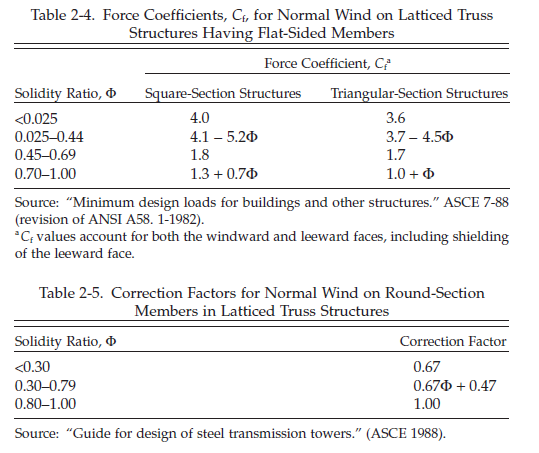
\includegraphics[width=\textwidth]{force_coefficient.png}
\caption{风压系数}\label{fig:force-coefficient}
\end{figure}
方形截面的风压系数根据图\ref{fig:force-coefficient}中Table 2-4计算,圆形截面的风压系数根据Table 2-4的系数再乘上Table 2-5中的系数。

\subsection{中国架空输电线路设计规范风荷载计算方法}
中国《110~750kV架空输电线路设计规范》\cite{GB50545-2010}中杆塔风荷载的计算公式为:
\begin{equation}
W_{\mathrm{s}} = W_{0} \cdot \mu_{\mathrm{z}} \cdot \mu_{\mathrm{s}} \cdot B_{2} \cdot A_{\mathrm{s}} \cdot \beta_{\mathrm{z}}
\end{equation}
\begin{equation}
W_0 = V^2/1600
\end{equation}
式中:
\begin{description}[leftmargin=!,labelwidth=2em]
\item[$W_{\mathrm{s}}$] 杆塔风荷载标准值(\SI{}{kN});
\item[$W_{0}$] 基准风压标准值(\SI{}{kN/m^2});
\item[$V$] 基准高度为\SI{10}{m}的风速(\SI{}{m/s});
\item[$\mu_{\mathrm{z}}$] 风压高度变化系数
\item[$\mu_{\mathrm{s}}$] 构件的体型系数,杆塔取$1.3(1+\eta)$,环形截面钢筋混凝土杆取$0.7$;
\item[$B_{2}$] 杆塔构件覆冰风荷载增大系数,\SI{5}{mm}冰区取$1.1$,\SI{10}{mm}冰区取$1.2$,\SI{15}{mm}冰区取$1.6$,\SI{20}{mm}冰区取$1.8$,\SI{20}{mm}以上冰区取$2.0$~$2.5$;
\item[$A_\mathrm{s}$] 迎风面构件的投影面积计算值(\SI{}{m^2});
\item[$\eta$] 塔架背风面荷载降低系数,按表\ref{tab:eta}选用;
\item[$\beta_\mathrm{z}$] 杆塔风荷载调整系数。
\end{description}

\begin{table}[!htbp]
\caption{塔架背风面荷载降低系数$\eta$}
\label{tab:eta}
\centering
\begin{tabu} to 1.0\textwidth {X[2,c] | X[c] X[c] X[c] X[c] X[c] X[c] }
  \toprule
  \diagbox{$b/a$}{$A_s/A$} & $\leq$ 0.1 & 0.2 & 0.3 & 0.4 & 0.5 & $>$ 0.6 \\
  \midrule
  $\leq$ 1 & 1.0 & 0.85 & 0.66 & 0.50 & 0.33 & 0.15 \\
  2 & 1.0 & 0.90 & 0.75 & 0.60 & 0.45 & 0.30 \\
  \bottomrule
\end{tabu}
\end{table}

\subsection{中美规范计算输电塔龙卷风荷载参数取值}
美国输电塔荷载规范Guidelines for electrical transmission line structural loading\cite{wong2009guidelines}针对输电塔受到的龙卷风风荷载的建议为:考虑F2等级的龙卷风荷载,因为F2等级龙卷风发生的概率较高,且能够在经济投入允许的情况下加以设防;由于龙卷风风场速度为阵风风速,故风速压力暴露系数$K_\mathrm{z}$和阵风系数$G$取为$1.0$,即利用龙卷风风场的实际风速代入公式计算,不利用系数$K_\mathrm{z}$对其进行修正;由于龙卷风荷载是一种极端荷载情况,故考虑平均重现期的风荷载调整系数$\gamma_\mathrm{w}$取为$1.0$。

文献\cite{hamada2010finite}\cite{hamada2011behaviour}\cite{altalmas2014finite}等建议地形系数$K_\mathrm{zt}$取为$1.0$,因为龙卷风多发生在平坦开阔的平原。


参考美国输电塔荷载规范计算龙卷风荷载的参数取值建议,中国《110~750kV架空输电线路设计规范》的相关参数建议为:忽略覆冰荷载的影响,故杆塔构件覆冰风荷载增大系数取为$1.0$;忽略龙卷风的风振效应,将杆塔风荷载调整系数取为$1.0$。

\subsection{输电塔龙卷风荷载施加方法}
将输电塔分为多层,见图\ref{fig:tower-zone}所示,某具体层示意图见图\ref{fig:tower-zone-diagram}。
输电塔节点a,b,c和d上受到的龙卷风荷载的计算步骤如下:
\begin{figure}[!htbp]
\centering
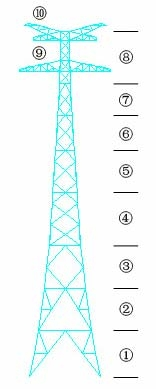
\includegraphics[width=0.3\textwidth]{tower_zone.jpg}
\caption{输电塔分层示意图}\label{fig:tower-zone}
\end{figure}

\begin{figure}[!htbp]
\centering
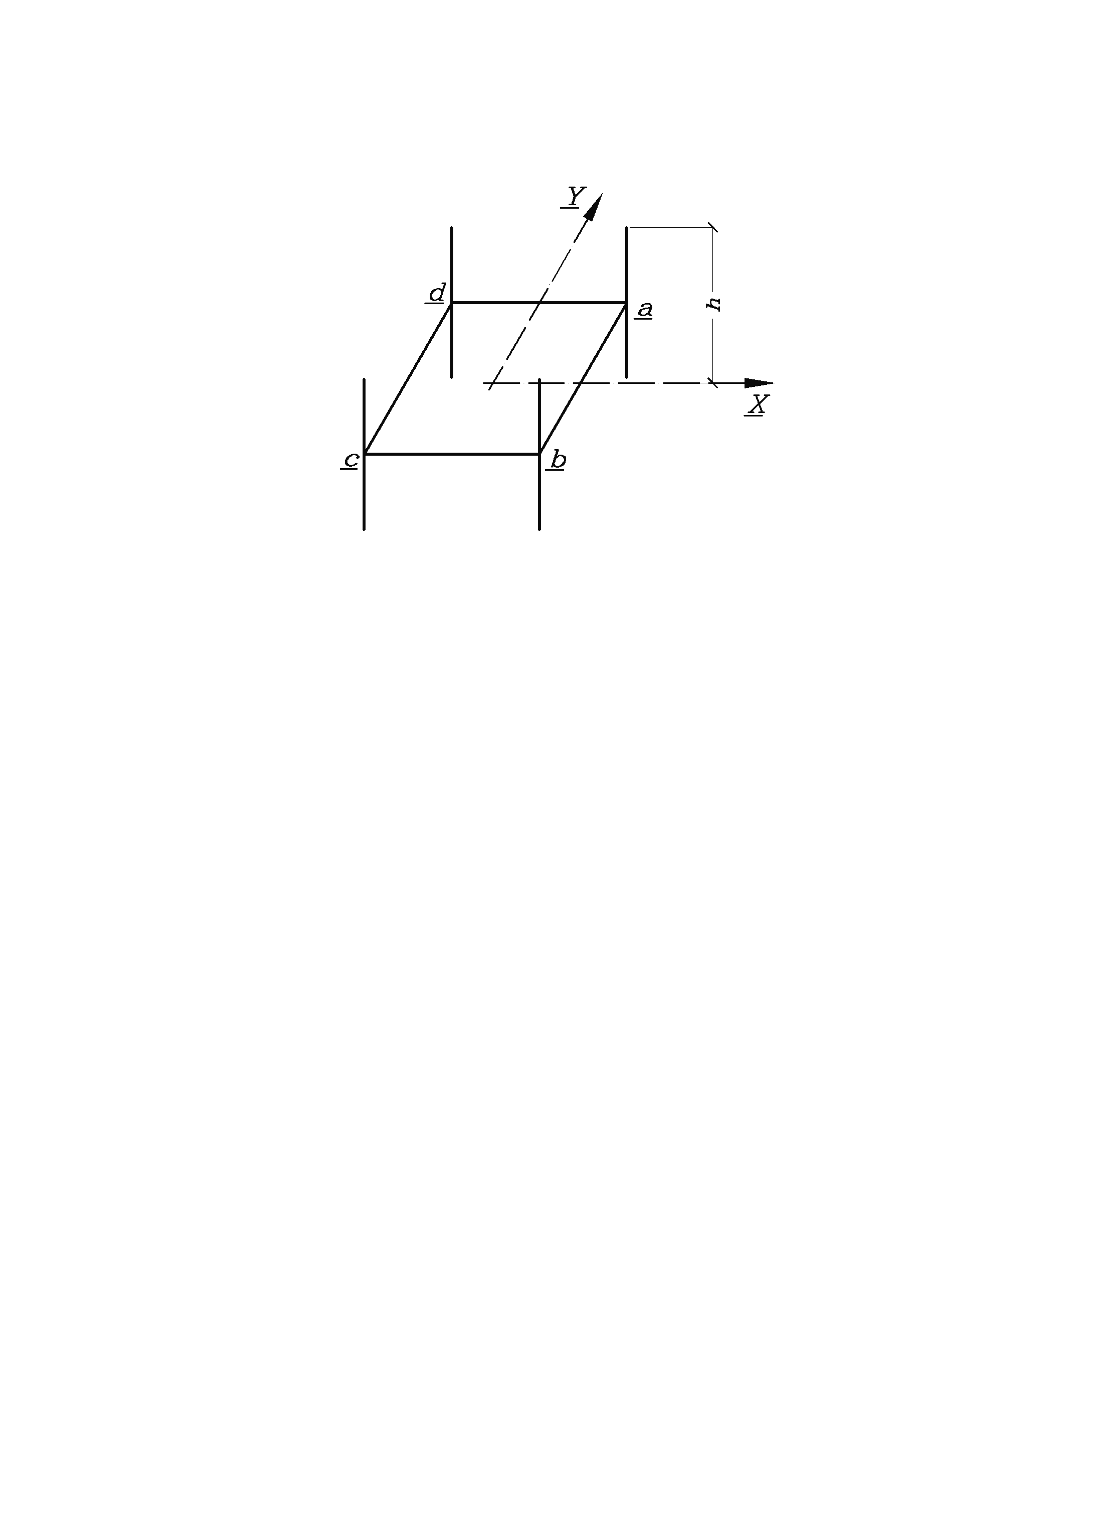
\includegraphics[width=0.6\textwidth]{tower_zone_diagram.pdf}
\caption{输电塔典型层示意图}\label{fig:tower-zone-diagram}
\end{figure}

\begin{enumerate}
\item 根据第\ref{sec:tornado}节计算输电塔节点a,b,c和d处龙卷风速度分量 $V_x$和$V_y$;
\item 分别沿$X$和$Y$方向计算风速风量的均值$V_x'$和$V_y'$;
\item 计算输电塔节点a,b,c和d处所在层龙卷风荷载,值得注意的是公式中各物理量采用SI单位制,即风速单位为\SI{}{m/s},风荷载单位为\SI{}{N}。

根据美国ASCE规范,该层$X$和$Y$方向龙卷风荷载$F_{\mathrm{w}x}$和$F_{\mathrm{w}y}$为
\begin{equation}
F_{\mathrm{w}x} = 0.613 (V_{x}')^2 C_{\mathrm{f}x} A_x
\end{equation}
\begin{equation}
F_{\mathrm{w}y} = 0.613 (V_{y}')^2 C_{\mathrm{f}y} A_y
\end{equation}
其中,$A_x$和$A_y$分别为该层迎风面构件沿$X$和$Y$方向的投影面积。
风压系数由\ref{fig:force-coefficient}计算。

根据中国规范,该层$X$和$Y$方向龙卷风荷载$F_{\mathrm{w}x}$和$F_{\mathrm{w}y}$为
\begin{equation}
F_{\mathrm{w}x} = 0.625 (V_{x}')^2 \mu_{\mathrm{s}x} A_x 
\end{equation}
\begin{equation}
F_{\mathrm{w}y} = 0.625 (V_{y}')^2 \mu_{\mathrm{s}y} A_y 
\end{equation}
体型系数$\mu_\mathrm{s} = 1.3(1+\eta)$,$\eta$由表\ref{tab:eta}计算。

可知中美规范计算龙卷风荷载的公式的主要区别如下:中国将风速转化为速度压的系数为$\SI{0.625}{kg/m^3}$,美国为$1/2\rho_a=\SI{0.613}{kg/m^3}$,中国规范稍微偏保守;二者的主要差别为体型系数(风压系数)的计算:对于圆形截面输电塔,$\Phi<0.025$的层,美国规范的风压系数为$C_\mathrm{f}=4.0\times0.67=2.68$,中国规范为$\mu_\mathrm{s}=1.3(1+\eta)=1.3 \times(1+1.0)=2.6$,相差不大,美国规范偏保守。

\item 迎风面和背风面上风荷载分配

中国规范根据塔架背风面荷载降低系数$\eta$对某层输电塔所受风荷载进行分配,即迎风面节点在$X$和$Y$方向所受风荷载分量分别为 $1/(1+\eta) F_{\mathrm{w}x}$ 和 $1/(1+\eta) F_{\mathrm{w}y}$;背风面节点在$X$和$Y$方向所受风荷载分量分别为 $\eta/(1+\eta) F_{\mathrm{w}x}$ 和 $\eta/(1+\eta) F_{\mathrm{w}y}$;

\item 迎(背)风面节点间风荷载分配

迎(背)风面上的节点根据各节点的投影面积进行迎(背)风面上风荷载的分配。


\end{enumerate}


\section{索的悬链线理论及输电线作用于塔的荷载}

\subsection{索的悬链线理论基本假设}
索由高强钢丝集束而成,相对抗弯刚度很小,其受力特点可以认为是完全柔性。
在自重和张力作用下分析其线形和力学参数时,基本假设如下:
\begin{itemize}
\item
索是理想柔性,既不能受压也不能受弯;
\item
索的材料符合胡克定律;
\item
索的横截面积在外荷载作用下的变化量十分微小,可忽略不计。
\end{itemize}

为了确定重力作用下索的线形,以弦左端点为原点、竖直向上为Y轴正方向建立右手直角坐标系。
则索受到的重力沿Y轴负向。
假设单位长度索的质量恒定,且不随张力变化。

\begin{figure}[!htbp]
  \centering
  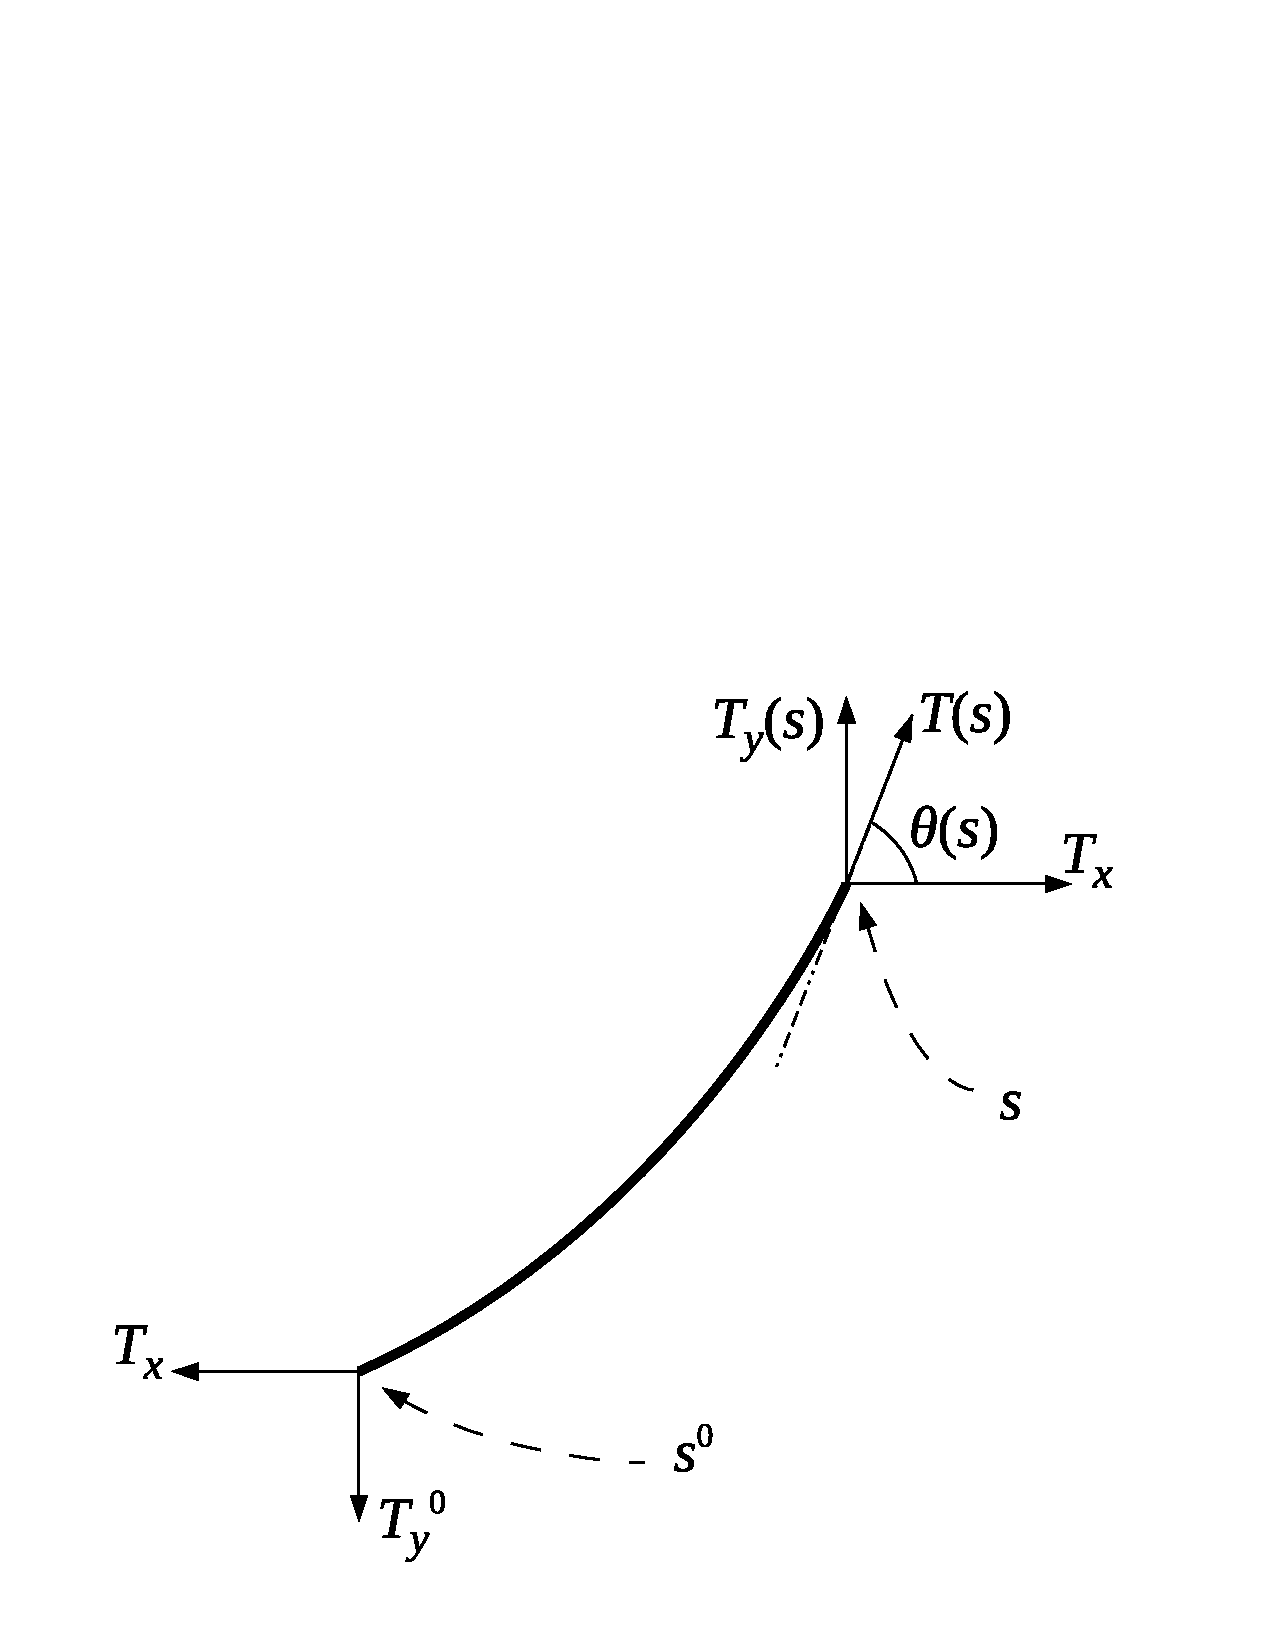
\includegraphics[width=0.6\textwidth]{catenary_diagram.pdf}
  \label{fig:catenary}
  \caption{索段计算示意图}
\end{figure}

\subsection{符号约定}
\begin{description}
  \item[$s$]
  从索左端点(坐标系原点)开始计算的索长度;
  \item[$\mu$]
  单位长度索的质量(假设是恒定的);
  \item[$T(s)$]
  索长度为$s$处的索张力(根据柔性索假设,张力沿索的切线方向);
  \item[$T_y(s)$]
  索长度为$s$处的索张力的$Y$向分量;
  \item[$T_x$]
  张力的$X$向分量(任取索段进行受力分析,由$X$向平衡方程可知$T_x$沿索长是均匀的);
  \item[$\theta(s)$]
  索切向量与$X$轴正向的夹角。
\end{description}

\subsection{自重作用下的单索线形求解}
索段竖向的平衡方程为:
\begin{gather}
  T_y(s) = g \int_{s^0}^{s} \mu \mathrm{d}s + T_y^0 \notag \\
  T_x \tan(\theta(s)) = g \mu \int_{s^0}^{s} \mathrm{d}s + T_y^0 \notag \\
  T_x \frac{\mathrm{d} y}{\mathrm{d} x} = g \mu \int_{s^0}^{s} \sqrt{1+\left(\frac{\mathrm{d} y}{\mathrm{d} x}\right)^2} \mathrm{d}x + T_y^0 \notag \\
  \frac{\mathrm{d}^2 y}{\mathrm{d} x^2} = \frac{g \mu}{T_x} \sqrt{1+\left(\frac{\mathrm{d} y}{\mathrm{d} x}\right)^2}
\end{gather}
此二阶微分方程的解析解为:
\begin{equation}
  y = \frac{T_x}{g \mu} \cosh \left( \frac{g \mu}{T_x} + c_1 \right)+c_2
\end{equation}
式中,$c_1$和$c_2$为由边界条件确定的积分常量。代入边界条件:$x=0,y=0;x=L,y=C$(见图\ref{fig:cat})。

\begin{figure}[!htpb]
\centering
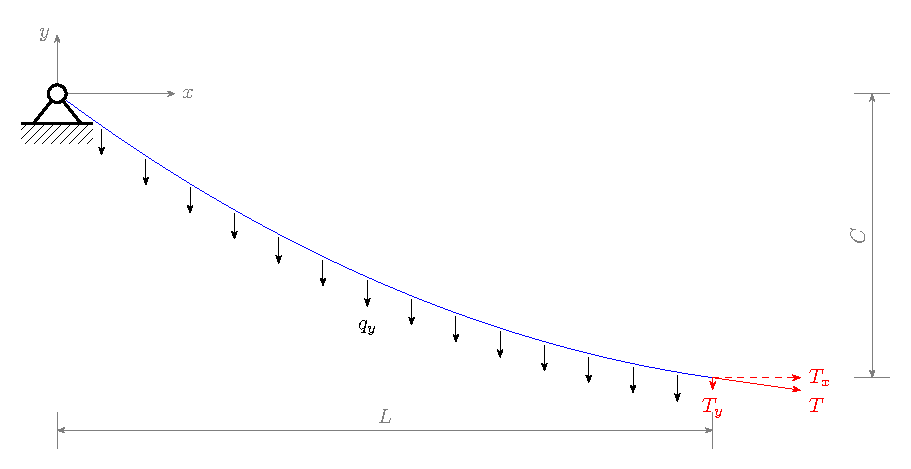
\includegraphics[width=0.8\textwidth]{cat.pdf}
\caption{单缆尺寸及边界条件示意图}
\label{fig:cat}
\end{figure}

\begin{equation}
  \left \{
    \begin{split}
      & \beta = \frac{g \mu L}{2 T_x}\\
      & c_1 = \sinh^{-1}\left(\frac{\beta C / L}{\sinh \beta}\right)\\
      & c_2 = -\frac{T_x}{g \mu} \cosh(c_1)
    \end{split}
  \right.
\end{equation}

悬链线索的形状长度$S$和无应力长度$S_0$分别为:
\begin{equation}
  S = \frac{T_x}{g\mu}\left[\sinh\left(\frac{g \mu L}{T_x}+c_1\right)+\sinh(c_1)\right]
\end{equation}

\begin{equation}
\begin{split}
  S_0 &= S-\Delta S \\
      &= S - \frac{T_x}{EA g \mu }\left[ \frac{1}{2} g \mu L + \frac{1}{8} T_x \left( e^{2(c_1+2\beta)} - e^{-2(c_1-2\beta)} -e^{2c_1} + e^{-2c_1} \right) \right]
\end{split}
\end{equation}

\subsection{输电线施加在输电塔的荷载求解}

跨越塔之间输电线跨度为$L=\SI{1770}{m}$,右侧支座比左侧支座高度相同,即$C=\SI{0}{}$,跨中矢高$f=\SI{132.4}{m}$,单位长度质量$\mu=\SI{3219}{kg/km}$。
索的弹性模量$E=\SI{108070}{MPa}$,截面积$A=\SI{729}{mm^2}$。
假设在外荷载作用下两支座的间距及高差保持不变。
主要任务是利用上述悬链线理论计算输电线对输电塔施加的荷载。

主要思路:输电线在自重和张力作用下,其线形为悬链线,故可采用悬链线经典公式来进行求解。
采用直接建模的方式,单缆采用LINK1单元模拟,单元水平长度为\SI{1}{m}。
分析时,首先假定水平力大小,根据悬链线方程求解节点坐标,由此建立节点和单元,并分析单缆在自重作用下的内力和线形。
如果求解获得的水平力与假定水平力之间的误差较大或者单缆变形较大,则返回重新计算,直至满足误差要求。计算框图如图\ref{fig:flow-chart}所示。
\begin{figure}[!htpb]
\centering
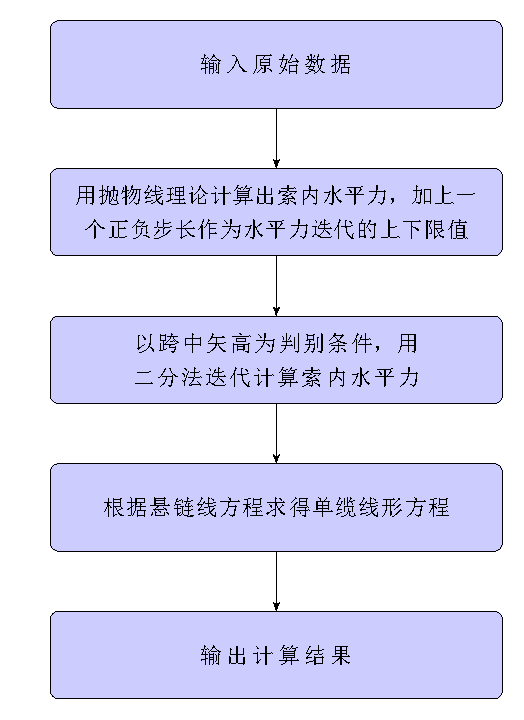
\includegraphics[width=0.4\textwidth]{flow_chart.pdf}
\caption{单缆线形和力学参数计算框图}
\label{fig:flow-chart}
\end{figure}

计算的APDL和MATLAB程序见附录\ref{apen:cat}。如图\ref{fig:cat-disp}所示,\SI{12.7}{mm},相比于跨径$L=\SI{1770}{m}$该变形已足够小,认为已满足精度要求。

\begin{figure}[!htbp]
\centering
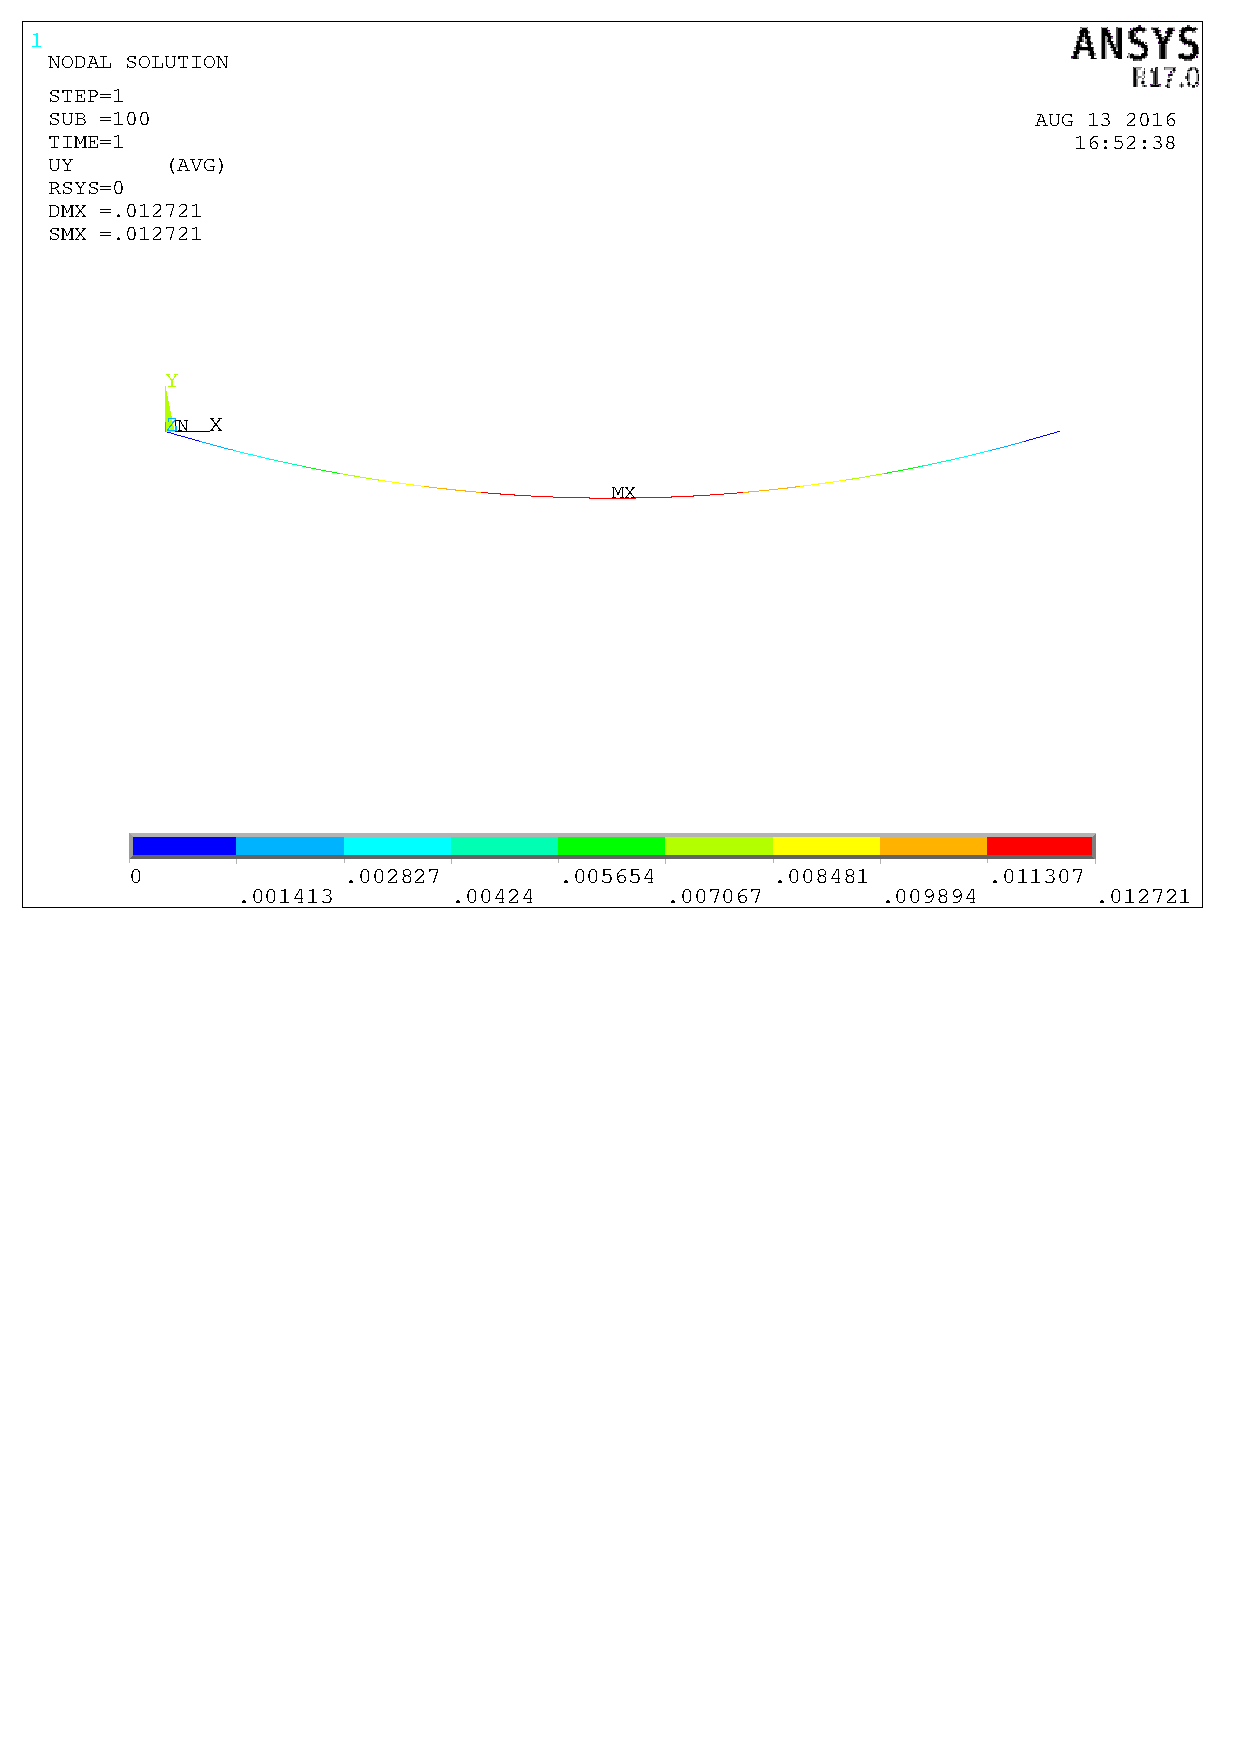
\includegraphics[width=0.8\textwidth]{cat_disp.pdf}
\caption{跨越塔之间输电线变形图(单位:\SI{}{m})}
\label{fig:cat-disp}
\end{figure}

对于跨越塔和锚塔之间的输电线对跨越塔的荷载计算采用相同的方法,在此不一一列举。

跨越塔受到的两侧输电线传来的张力的示意图见图\ref{fig:line-force}所示。

\begin{figure}[!htbp]
\centering
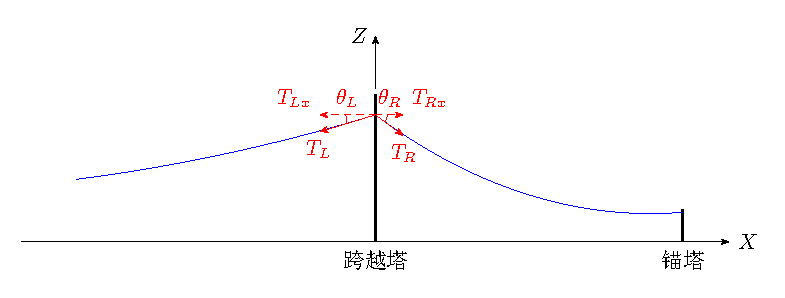
\includegraphics[width=0.8\textwidth]{line_force}
\caption{跨越塔受到输电线的张力示意图}
\label{fig:line-force}
\end{figure}

经过附录\ref{apen:cat}程序的计算,图\ref{fig:line-force}中各量为:
\begin{equation}
\begin{split}
  T_{Lx} & = \SI{93.31}{kN},\quad \theta_L  = \ang{16.89} \\
  T_{Rx} & = \SI{21.33}{kN},\quad \theta_L  = \ang{36.70}
\end{split}
\end{equation}



\section{龙卷风位置变化的参数分析}
\subsection{位移响应参数化分析}
利用附录\ref{apen:static}中的APDL程序进行龙卷风作用下输电塔结构的静力响应分析,
并改变龙卷风核心位置$(R, \theta)$(见图\ref{fig:tower-tornado-cs}),
分析其对输电塔塔顶位移响应的影响,如表\ref{tab:disp}和图\ref{fig:disp}所示。

\begin{table}[!htbp]
  \centering
  \caption{塔顶位移响应(\SI{}{mm})随龙卷风核心位置的参数化分析}
  \label{tab:disp}
  \begin{tabu} to 1.0\textwidth {X[1.5,c] X[1,r] X[1,r] X[1,r] X[1,r] X[1,r] X[1,r] X[1,r]}
    \toprule
    \diagbox{$R/\SI{}{m}$}{$\theta/\SI{}{\degree}$} & 0 & 15 & 30 & 45 & 60 & 75 & 90 \\
    \midrule
    500 &  377.3 & 434.4 &  537.1 &  607.8 &  430.5 &  459.3 &  367.5 \\
    450 &  425.1 & 475.6 &  601.5 &  674.6 &  465.9 &  509.5 &  411.1 \\
    400 &  479.1 & 517.4 &  675.1 &  743.4 &  502.6 &  563.2 &  459.9 \\
    350 &  542.6 & 560.2 &  763.1 &  814.3 &  542.5 &  621.6 &  517.9 \\
    300 &  629.4 & 611.6 &  886.2 &  898.1 &  596.7 &  694.5 &  602.1 \\
    250 &  775.4 & 699.7 & 1092.5 & 1027.3 &  700.6 &  811.8 &  755.6 \\
    200 & 1001.8 & 842.8 & 1403.9 & 1199.9 &  885.5 &  984.1 & 1010.8 \\
    150 & 1139.5 & 920.6 & 1567.2 & 1232.6 & 1016.9 & 1063.0 & 1175.6 \\
    120 & 1042.8 & 823.9 & 1394.7 & 1035.9 &  942.6 &  952.0 & 1059.3 \\
    100 &  794.7 & 626.0 & 1105.3 &  756.2 &  736.0 &  710.3 &  843.8 \\
    \bottomrule
  \end{tabu}
\end{table}
可知,塔顶位移响应的危险工况位于$\theta=\SI{30}{\degree}$附近,
且径向位置靠近核心半径$r_c=\SI{120}{m}$处。

\begin{figure}[!htbp]
  \centering
  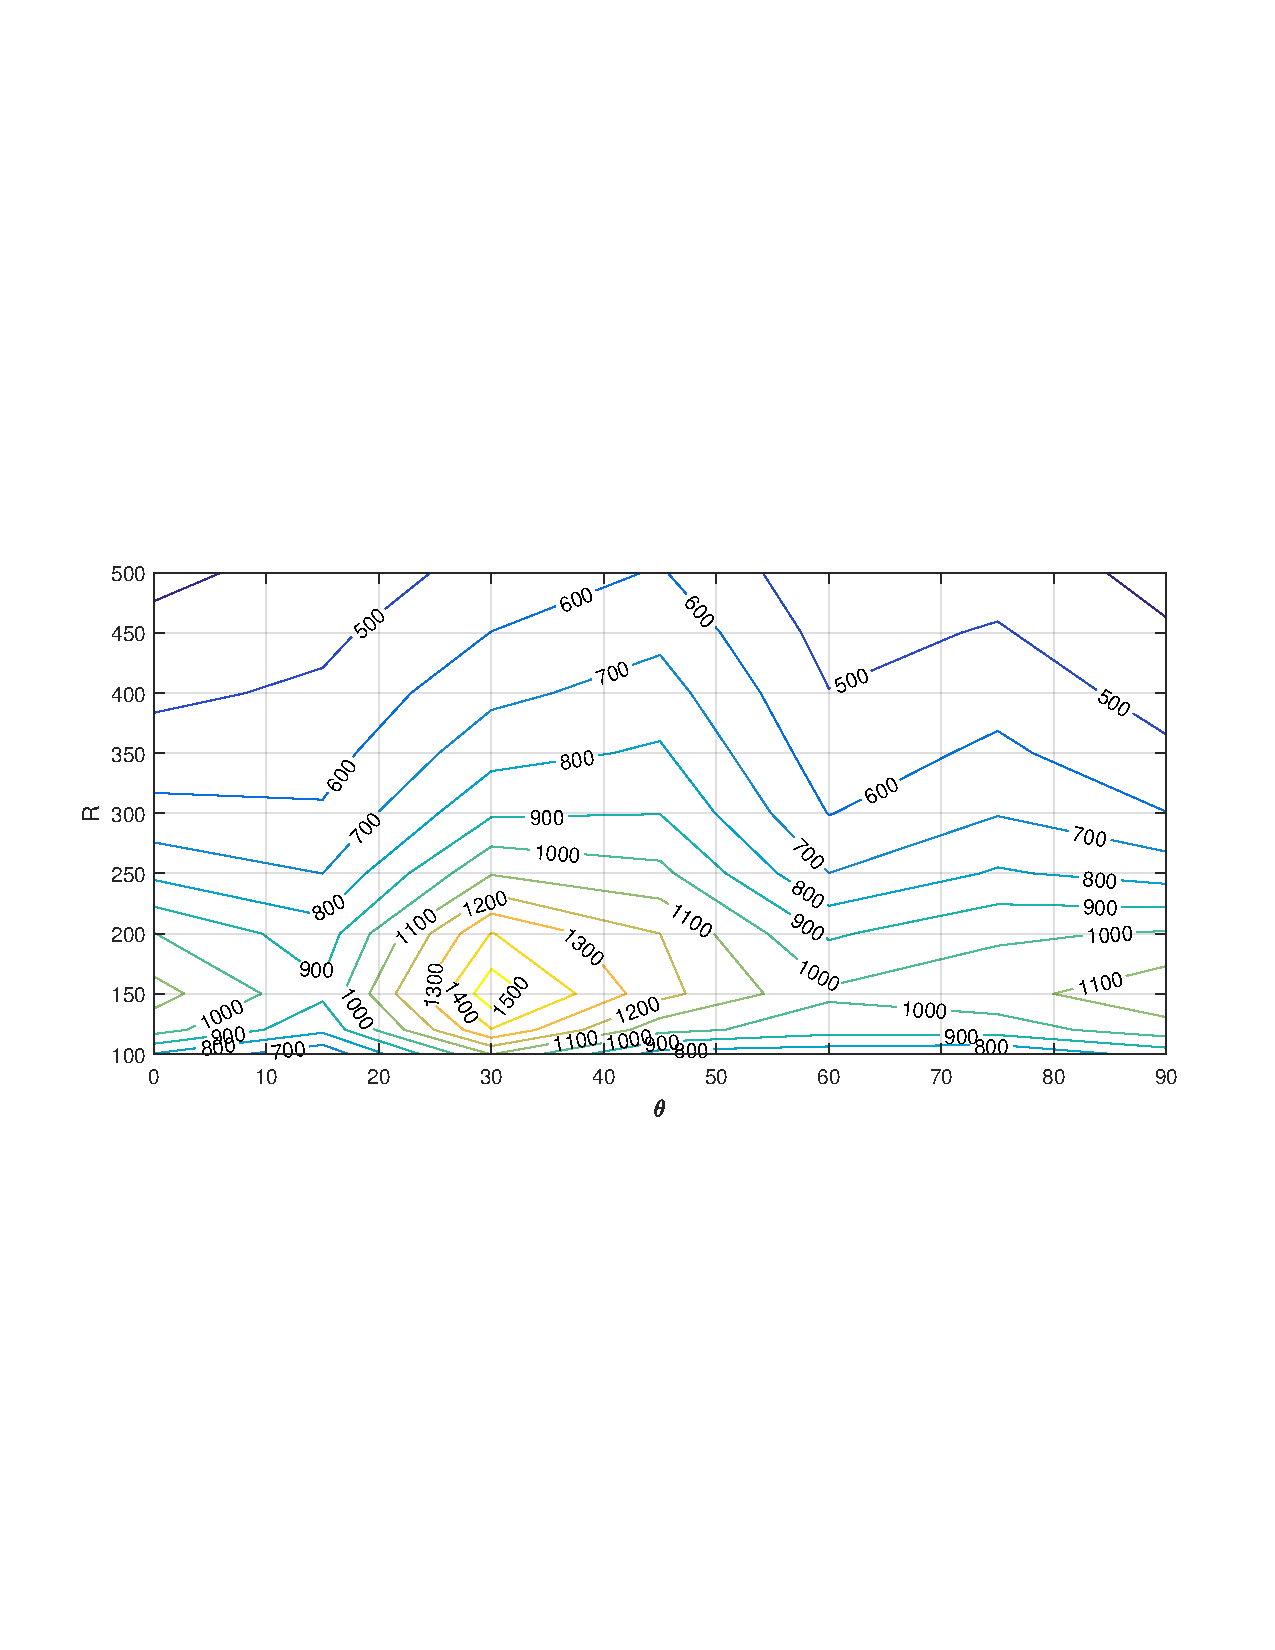
\includegraphics[width=1.0\textwidth]{disp.pdf}
  \caption{输电塔位移响应随龙卷风核心位置变化的等值线图}
  \label{fig:disp}
\end{figure}

\graphicspath{{figures/dynamic/}}

\chapter{考虑龙卷风平移的动态响应分析}

第\ref{chapter:static}章忽略了龙卷风平移运动的影响,
分别在\SI{0}{\degree}、\SI{45}{\degree}和\SI{90}{\degree}工况下进行静力非线性分析。
本章考虑龙卷风平移运动的影响,假定其移动轨迹后计算输电塔结构各节点荷载时程,
进行动力时程分析,分析其动态响应。

\section{动态龙卷风模型}

根据第\ref{sec:tower-fea}建立整体坐标系,如图\ref{fig:tower-tornado-cs}所示。
龙卷风相应于输电塔结构做平移运动的示意图见图\ref{fig:tornado-path}\todo{replot}所示。
\begin{figure}[!htpb]
	\centering
	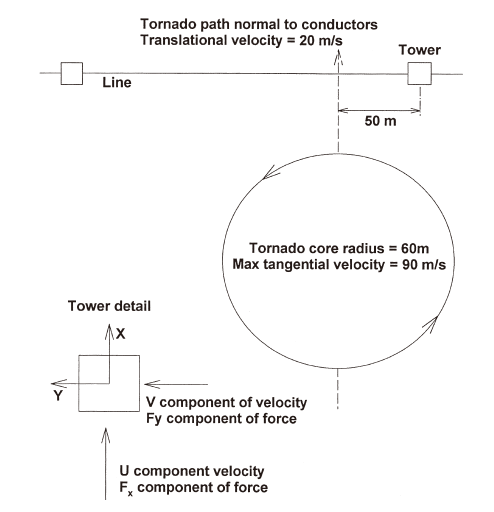
\includegraphics[width=0.6\textwidth]{tornado-path.png}
	\caption{龙卷风相应于输电塔做平移运动的示意图}
	\label{fig:tornado-path}
\end{figure}

\subsection{龙卷风路径}

假定龙卷风核心在地面上做匀速直线运动,描述其路径的关键参数为核心初始位置和运动速度。

为了使得初始时刻输电塔结构所受龙卷风荷载较小,需要将龙卷风核心初始位置设置在距离输电塔较远的地方。
若初始时刻龙卷风核心距离输电塔很近,结构会受到量值很大的突加荷载的影响,与实际情况不符。
初始位置在整体坐标系中的位置记为$\left(x^T_{0},y^T_{0}\right)$。

关于龙卷风的平移速度在第\ref{sec:tornado-cha}节已有介绍,
我国《三十万千瓦压水堆核电厂安全重要土建结构抗龙卷风设计规定》中A类龙卷风平移速度为\SI{22.4}{m/s},
文献\cite{savory2001modelling}\cite{hamada2011behaviour}中选用龙卷风平移速度为\SI{20.0}{m/s},
二者差别较小,本文为计算简便选用$v^T=\SI{20.0}{m/s}$。
确定龙卷风路径还需龙卷风平移速度的方向,设平移速度相对于输电线、即$X$轴正向的夹角为$\theta^T$。

综上,龙卷风运动轨迹$\left(x^T(t),y^T(t)\right)$可表示为:
\begin{equation}
	\begin{cases}
		x^T(t) = x^T_0 + \left(v^T\cos{\theta^T}\right)t \\
		y^T(t) = y^T_0 + \left(v^T\sin{\theta^T}\right)t 
	\end{cases}
\end{equation}
龙卷风的平移运动引起了龙卷风核心相对输电塔位置$\left(x^T(t),y^T(t)\right)$随时间变化,
进而使得输电塔受到了随龙卷风位置变化的荷载时程,需进行动力时程分析计算结构响应。

本文假设龙卷风风场结构不随时间变化(实际中龙卷风会随其运动衰减,本文忽略这一现象),
即采用第\ref{sec:full-tornado}中模拟的足尺龙卷风风场作为任一时刻动态龙卷风的风场。

\section{动态龙卷风风速及荷载时程}

在任意时刻$t$,利用第\ref{sec:static-code}节中规范方法施加该时刻的龙卷风荷载。
由于第\ref{sec:static-code}节已编制了计算龙卷风荷载并施加到输电塔结构的APDL程序,
在动力分析中,改变龙卷风核心相应于输电塔中心的极坐标$(R,\theta)$(见第\ref{sec:d-polor}节),
调用龙卷风荷载施加子程序,即可完成动态荷载施加过程。

输电塔结构在龙卷风时变荷载作用下的动态响应由动力时程分析计算。
时间步长选用\SI{0.10}{s}。
并进行时间步长的敏感性分析,发现当时间步长减小为\SI{0.05}{s}时结构动态响应差别较小。
这说明\SI{0.10}{s}的时间步长是足够精确的。

\subsection{典型龙卷风运动工况}

龙卷风平移运动的两种典型工况见图\ref{fig:dynamic-case1}和图\ref{fig:dynamic-case2}。
图\ref{fig:dynamic-case1}中龙卷风运动路径平行于输电线,下文简称为龙卷风平行运动工况;
图\ref{fig:dynamic-case2}中龙卷风运动路径垂直于输电线,下文简称为龙卷风垂直运动工况。

\begin{figure}[!htpb]
    \centering
    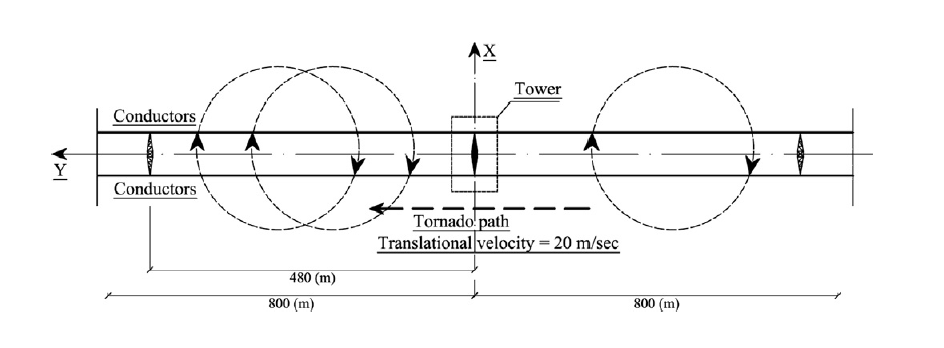
\includegraphics[width=0.8\textwidth]{dynamic-case1.png}
    \caption{龙卷风平行运动工况}
    \label{fig:dynamic-case1}
\end{figure}
\begin{figure}[!htpb]
    \centering
    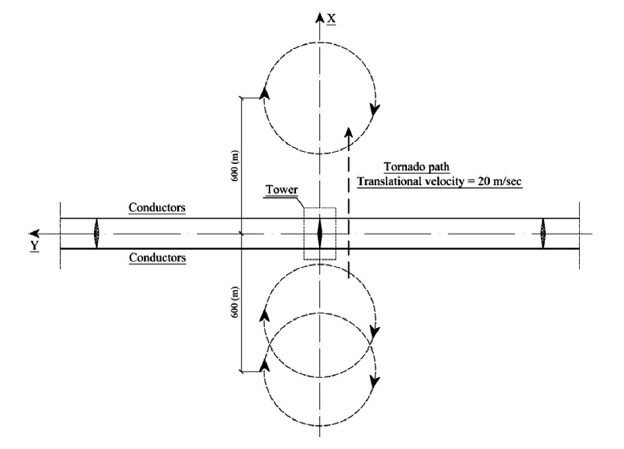
\includegraphics[width=0.8\textwidth]{dynamic-case2.png}
    \caption{龙卷风垂直运动工况}
    \label{fig:dynamic-case2}
\end{figure}

平行运动工况(图\ref{fig:dynamic-case1})中,
龙卷风核心初始位置选为$x_0^T=\SI{1500}{m}$,$y_0^T=\SI{120}{m}$;
平移速度$v^T=\SI{20.0}{m/s}$,$\theta^T=\pi$。
满足初始时刻龙卷风距离输电塔较远,龙卷风荷载较小,
且在运动过程二者距离取得龙卷风核心半径$r_c=\SI{120}{m}$,受到龙卷风荷载较大。

类似选取垂直运动工况(图\ref{fig:dynamic-case2})的参数,
龙卷风核心初始位置选为$x_0^T=\SI{120}{m}$,$y_0^T=\SI{1500}{m}$;
平移速度$v^T=\SI{20.0}{m/s}$,$\theta^T=-\frac{1}{2}\pi$。

\subsection{动态龙卷风风速时程}

\subsection{动态龙卷风荷载时程}

\section{输电塔结构动态时程分析}


\thesisbib{seuthesix}

% \acknowledgement
% 感谢每一个给予帮助的人。


\appendix
\chapter{龙卷风数值模拟速度入口处边界条件的UDF程序}\label{apen:udf}
\begin{minted}{c}
#include "udf.h"

#define H 0.4
#define R 0.4
#define UREF 0.34    /* reference velocity */
#define ZREF 0.025    /* reference height */
#define S 0.28    /* swirl ratio */

/* profile for radial velocity */
DEFINE_PROFILE(V_r, t, i)
{
    real x[ND_ND], z;
    face_t f;

    begin_f_loop(f, t)
    {
        F_CENTROID(x, f, t);
        z = x[2];
        F_PROFILE(f, t, i) = -UREF*pow(z/ZREF,1.0/7.0);
    }
    end_f_loop(f, t)
}

/* profile for tangential velocity */
DEFINE_PROFILE(V_t, t, i)
{
    real x[ND_ND], z;
    face_t f;

    begin_f_loop(f, t)
    {
        F_CENTROID(x, f, t);
        z = x[2];
        F_PROFILE(f, t, i) = 2.0*S*UREF*pow(z/ZREF,1.0/7.0);
    }
    end_f_loop(f, t)
}

\end{minted}

\chapter{计算输电线对输电塔荷载的APDL和MATLAB程序}\label{apen:cat}
\section{计算跨越塔之间输电线对跨越塔水平荷载的 ANSYS APDL 命令流}

\begin{minted}{apdl}

! UNITS: m-kN
FINISH
/CLEAR
/PREP7
EA=729E-6                                ! 单缆面积(m^2)
EE=1.0807E8                              ! 弹性模量(kN/m^2)
QQ=0.0315462                             ! 单缆每延米重量(kN/m)
YSM0=132.4                               ! 中跨矢高(m)
CH=0                                     ! 中跨锚点高差(m)
SPAN=1770                                ! 跨径
                                         
ET,1,LINK1                               ! 定义单元
R,1,EA,1.0E-5                            ! 设置一个较小的初应变
MP,EX,1,EE                               ! 定义材料特性
MP,PRXY,1,0.3
MP,DENS,1,43.273

! 根据抛物线理论计算水平力迭代初始值
FF=YSM0-CH/2
HH=QQ*SPAN**2/(8*FF)                     ! 计算水平力
HH1=0.9*HH                               ! 设置水平力迭代区间
HH2=1.1*HH

! 用二分法迭代计算主缆水平力
*DO,I,1,100,1
    HFM=(HH1+HH2)/2                      ! 水平力迭代初值
    CI=QQ/HFM                            ! 中间参数
    A0=CH*CI/SINH(SPAN*CI/2)/2           ! 中间参数
    AI=LOG(A0+SQRT(A0**2+1))+SPAN*CI/2   ! 中间参数alpha
    BI=COSH(AI)/CI                       ! 中间参数alpha1
    YSM=BI-COSH(CI*(SPAN/2)-AI)/CI       ! 计算跨中矢高
    *IF,YSM,GT,YSM0,THEN                 ! 修正水平力
        HH1=HFM
    *ELSEIF,YSM,LE,YSM0
        HH2=HFM
    *ENDIF
*ENDDO
ERROR1=(YSM-YSM0)/YSM0                   ! 跨中处索垂度误差
MSS=(SINH(CI*SPAN-AI)+SINH(AI))/CI       ! 按悬链线方程得出的形状长度
DSO=HFM*(SPAN+(SINH(2*CI*SPAN-2*AI)+SINH(2*AI))/2/CI)/(2*EE*EA)
                                         ! 按悬链线方程得出的伸长量
YBM=DSO/(MSS-DSO)                        ! 中跨的初始应变
R,1,EA,YBM                               ! 修改单缆初始应力
EL=1 ! 单元水平长度
ENU=SPAN/EL+1
*DIM,X,ARRAY,ENU,1
*DIM,Y,ARRAY,ENU,1
*DO,I,1,ENU,1                            ! 定义单缆节点
    X(I)=(I-1)*EL
    Y(I)=BI-COSH(CI*X(I)-AI)/CI
    N,I,X(I),-Y(I),0
*ENDDO
TYPE,1
MAT,1
REAL,1
ESYS,0                                    ! 单缆单元
*DO,I,1,ENU-1,1
    E,I,I+1
*ENDDO
EPLOT
FINISH

/SOLU
D,1,ALL                                   ! 定义边界条件
D,ENU,ALL
ACEL,0,1,0                                ! 施加重力荷载
ANTYPE,STATIC
NLGEOM,ON
NROPT,AUTO
LUMPM,OFF
EQSLV,,,0
AUTOTS,OFF
NSUBST,100

KBC,0

ALLSEL
SOLVE

/POST1
PLNSOL,U,Y

\end{minted}

\section{计算跨越塔之间输电线对跨越塔竖向荷载的 MATLAB 程序}
\begin{minted}{matlab}
L = 1770;
C = 0;
q_y = 0.0315462;
Tx = 93.3072979;
beta = q_y*L/(2*Tx);
c1 = asinh((beta*C/L)/sinh(beta))-beta;
c2 = -Tx/q_y*cosh(c1);
cat = @(x) Tx/q_y*cosh(q_y/Tx*x+c1)+c2;
cat_d = @(x) sinh(q_y/Tx*x+c1);
x = 0:L;
y = cat(x);
csvwrite('cat.csv',horzcat(transpose(x/100), transpose(y/100)))
mid_def = cat(L/2);
theta = cat_d(L);
plot(x,y)
hold on
axis equal

\end{minted}
\graphicspath{{figures/static/}}
\chapter{输电塔结构在龙卷风作用下的静态响应分析}\label{chapter:static}

本章主要进行输电塔结构在龙卷风作用下的静态响应分析,即忽略龙卷风的平移效应,选定龙卷风核心相应于输电塔结构中心的位置,进行静力弹塑性分析。输电塔结构受到的主要荷载为:
\begin{enumerate}
\item 重力荷载
\item 输电塔受到的龙卷风涡旋风场的荷载
\item 输电线传到输电塔的荷载
\end{enumerate}
其中忽略了龙卷风对输电线的荷载,主要是因为:
\begin{enumerate}
\item 龙卷风路径宽度较小,F1-F2级龙卷风的路径宽度为\SI{60}{m}-\SI{150}{m}。
\item 输电线受到的风荷载作用机制比较复杂。
\end{enumerate}


\section{龙卷风风场处理}\label{sec:tornado}
输电塔在龙卷风风场中的水平投影示意图如图\ref{fig:tower-tornado-cs}所示。
\begin{figure}[!htpb]
  \centering
  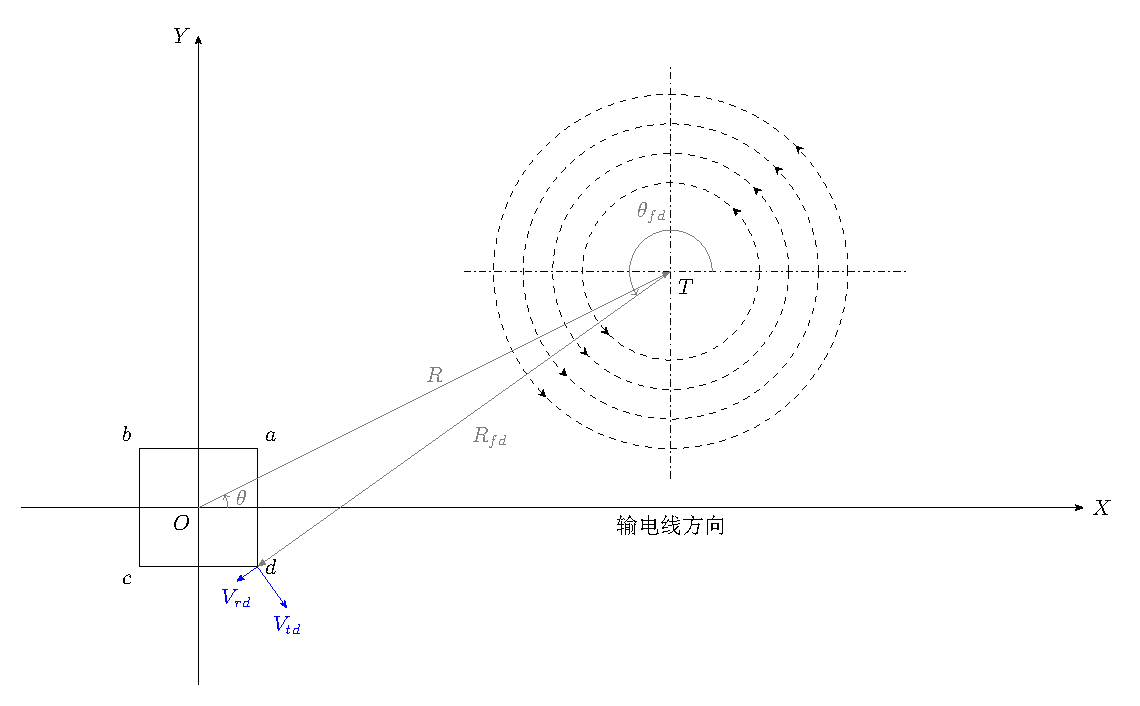
\includegraphics[width=\textwidth]{tower_tornado_cs.pdf}
  \caption{输电塔在龙卷风风场中的水平投影示意图}
  \label{fig:tower-tornado-cs}
\end{figure}
输电塔直角坐标系$\{O: XYZ\}$的建立方法见第\ref{sec:tower-fea}节。
$abcd$为输电塔处于同一水平剖面的节点。
下文主要展示推导$d$节点处龙卷风风速的方法,其余节点类似。
龙卷风中心在坐标系$\{O: XYZ\}$中的位置用极坐标$(R, \theta)$表示。
输电塔节点$d$相应于龙卷风核心的极坐标为$(R_{fd}, \theta_{fd})$,$d$节点受到的龙卷风切向、径向风速分别为$V_{td}$、$V_{rd}$,以及图\ref{fig:tower-tornado-cs}未明确表示的竖向风速$V_{ad}$。

\subsection{输电塔节点相应于龙卷风中心位置的极坐标}\label{sec:d-polor}
假设$d$节点在输电塔坐标系$\{O: XYZ\}$中的坐标为$(x_d, y_d, z_d)$,下文将推导节点$d$相应于龙卷风中心的极坐标$(R_{fd}, \theta_{fd})$。

龙卷风中心$T(R, \theta)$在输电塔坐标系$\{O: XYZ\}$中的直角坐标为$(R\cos\theta, R\sin\theta)$,则节点$d$相应于龙卷风中心$T$的向量为:
\begin{equation}
  \vv{Td} = \vv{Od} - \vv{OT} = (x_d - R\cos\theta, y_d - R\sin\theta) = R_{fd}(\cos\theta_{fd}, \sin\theta_{fd})
\end{equation}
式中,
\begin{equation}
\begin{split}
  R_{fd} & = \sqrt{(x_d-R\cos\theta)^2+(y_d-R\sin\theta)^2} \\
  \theta_{fd} & = \arctan \frac{y_d - R\sin\theta}{x_d - R\cos\theta}
\end{split}
\end{equation}

\subsection{龙卷风风场在直角坐标系下的分量}\label{sec:cs}
第\ref{sec:tornado}节模拟的龙卷风风场是定义在极坐标系下的,而施加风荷载采用直角坐标系下的风速分量较为简单,因此需要将龙卷风风场从极坐标系转化为直角坐标系。

输电塔节点$d$受到的龙卷风径向风速$V_{rd}$与$X$轴正方向的夹角为$\theta_{fd}$(图\ref{fig:tower-tornado-cs}),切向风速$V_{td}$与$X$轴正方向的夹角为$(\theta_{fd}+\pi/2)$,进行速度的分解如下:
\begin{equation}
\begin{split}
  V_{xd} & = V_{rd} \cos\theta_{fd} + V_{td} \cos(\theta_{fd}+\pi/2) \\
         & = V_{rd} \cos\theta_{fd} - V_{td} \sin(\theta_{fd}) \\
  V_{yd} & = V_{rd} \sin\theta_{fd} + V_{td} \sin(\theta_{fd}+\pi/2) \\
         & = V_{rd} \sin\theta_{fd} + V_{td} \cos(\theta_{fd}) \\   
  V_{zd} & = V_{ad}  
\end{split}
\end{equation}

有了上述准备工作,就可以计算输电塔上任意节点受到的龙卷风风速在直角坐标系下的分量了。

\subsection{龙卷风风场中任意节点处风速分量}
输电塔节点$d$相应于龙卷风中心的实际位置为$(R_{fd}, \theta_{fd})$(见第\ref{sec:d-polor}节),此节点对应于缩尺龙卷风风场$V_r(r,z)$、$V_t(r,z)$和$V_a(r,z)$(见第\ref{sec:tornado}节)中的位置为$(R_{md}, Z_{md})$,且
\begin{equation}
\begin{split}
  R_{md} & = R_{fd} / L_s \\
  Z_{md} & = z_{fd} / L_s
\end{split}
\end{equation}

在缩尺龙卷风风场中,由位置$(R_{md}, Z_{md})$可提取缩尺龙卷风风场径向、切向和竖向风速分量分别为$V_{rmd}$、$V_{tmd}$和$V_{amd}$。根据缩尺龙卷风速度相似比$V_s$可将其转化为足尺龙卷风风场中的速度分量:

\begin{equation}
\begin{split}
  V_{rd} &= V_{rmd} \times V_s \\
  V_{td} &= V_{tmd} \times V_s \\
  V_{ad} &= V_{amd} \times V_s
\end{split}
\end{equation}

最后根据第\ref{sec:cs}节的方法即可将输电塔节点$d$受到的极坐标系下的足尺龙卷风风速分量转化为直角坐标系下的风速分量。


\section{输电塔结构龙卷风风荷载计算}

\subsection{ASCE输电塔荷载规范风荷载计算方法}
ASCE主编的输电塔荷载规范 Guidelines for electrical transmission line structural loading\cite{wong2009guidelines}中输电塔风荷载计算公式为:
\begin{equation}
F = \gamma_{\mathrm{w}} Q K_{\mathrm{z}} K_{\mathrm{zt}} \left( V_{50}\right)^2 G C_{\mathrm{f}} A
\end{equation}
其中:
\begin{description}[leftmargin=!,labelwidth=2em]
\item[$F$] 顺风向风荷载
\item[$\gamma_{\mathrm{w}}$] 考虑平均重现期的风荷载调整系数。平均重现期为$50$年时,$\gamma_{\mathrm{w}}=1.0$;平均重现期为$100$年时,$\gamma_{\mathrm{w}}=1.15$
\item[$V_{50}$] 平均重现期为$50$年规定的风速基准值(基本风速)
\item[$K_{\mathrm{z}}$] 风速压力暴露系数
\item[$K_{\mathrm{zt}}$] 地形系数
\item[$Q$] 将风速转化为速度压的常数,$Q=1/2 \rho_a=\SI{0.613}{kg/m^3}$
\item[$G$] 阵风系数
\item[$C_{\mathrm{f}}$] 风压系数
\item[$A$] 迎风面构件的投影面积
\end{description}
各量中文翻译参考刘刚的论文\cite{liu2010wind}。

下面介绍ASCE规范中输电塔结构所受风荷载的风压系数$C_{\mathrm{f}}$的计算方法。

风压系数是密实度系数(solidity ratio)$\Phi$的函数,定义为:
\begin{equation}
\Phi = \frac{A_\mathrm{m}}{A_\mathrm{o}}
\end{equation}
其中:
\begin{description}[leftmargin=!,labelwidth=2em]
\item[$A_\mathrm{m}$] 迎风面构件的投影面积
\item[$A_\mathrm{o}$] 塔架的轮廓面积
\end{description}
风压系数与密实度系数$\Phi$的关系表见图\ref{fig:force-coefficient}\cite{wong2009guidelines}
\begin{figure}[!htbp]
\centering
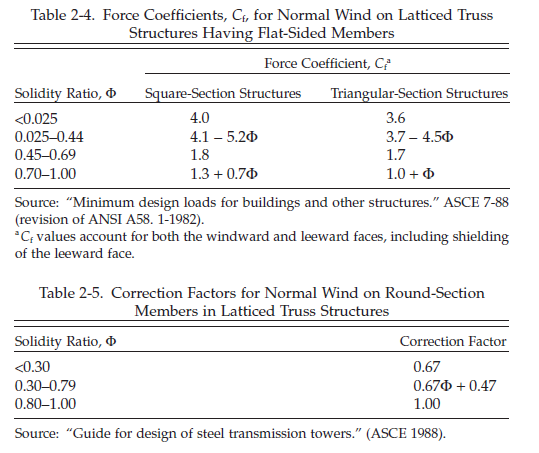
\includegraphics[width=\textwidth]{force_coefficient.png}
\caption{风压系数}\label{fig:force-coefficient}
\end{figure}
方形截面的风压系数根据图\ref{fig:force-coefficient}中Table 2-4计算,圆形截面的风压系数根据Table 2-4的系数再乘上Table 2-5中的系数。

\subsection{中国架空输电线路设计规范风荷载计算方法}
中国《110~750kV架空输电线路设计规范》\cite{GB50545-2010}中杆塔风荷载的计算公式为:
\begin{equation}
W_{\mathrm{s}} = W_{0} \cdot \mu_{\mathrm{z}} \cdot \mu_{\mathrm{s}} \cdot B_{2} \cdot A_{\mathrm{s}} \cdot \beta_{\mathrm{z}}
\end{equation}
\begin{equation}
W_0 = V^2/1600
\end{equation}
式中:
\begin{description}[leftmargin=!,labelwidth=2em]
\item[$W_{\mathrm{s}}$] 杆塔风荷载标准值(\SI{}{kN});
\item[$W_{0}$] 基准风压标准值(\SI{}{kN/m^2});
\item[$V$] 基准高度为\SI{10}{m}的风速(\SI{}{m/s});
\item[$\mu_{\mathrm{z}}$] 风压高度变化系数
\item[$\mu_{\mathrm{s}}$] 构件的体型系数,杆塔取$1.3(1+\eta)$,环形截面钢筋混凝土杆取$0.7$;
\item[$B_{2}$] 杆塔构件覆冰风荷载增大系数,\SI{5}{mm}冰区取$1.1$,\SI{10}{mm}冰区取$1.2$,\SI{15}{mm}冰区取$1.6$,\SI{20}{mm}冰区取$1.8$,\SI{20}{mm}以上冰区取$2.0$~$2.5$;
\item[$A_\mathrm{s}$] 迎风面构件的投影面积计算值(\SI{}{m^2});
\item[$\eta$] 塔架背风面荷载降低系数,按表\ref{tab:eta}选用;
\item[$\beta_\mathrm{z}$] 杆塔风荷载调整系数。
\end{description}

\begin{table}[!htbp]
\caption{塔架背风面荷载降低系数$\eta$}
\label{tab:eta}
\centering
\begin{tabu} to 1.0\textwidth {X[2,c] | X[c] X[c] X[c] X[c] X[c] X[c] }
  \toprule
  \diagbox{$b/a$}{$A_s/A$} & $\leq$ 0.1 & 0.2 & 0.3 & 0.4 & 0.5 & $>$ 0.6 \\
  \midrule
  $\leq$ 1 & 1.0 & 0.85 & 0.66 & 0.50 & 0.33 & 0.15 \\
  2 & 1.0 & 0.90 & 0.75 & 0.60 & 0.45 & 0.30 \\
  \bottomrule
\end{tabu}
\end{table}

\subsection{中美规范计算输电塔龙卷风荷载参数取值}
美国输电塔荷载规范Guidelines for electrical transmission line structural loading\cite{wong2009guidelines}针对输电塔受到的龙卷风风荷载的建议为:考虑F2等级的龙卷风荷载,因为F2等级龙卷风发生的概率较高,且能够在经济投入允许的情况下加以设防;由于龙卷风风场速度为阵风风速,故风速压力暴露系数$K_\mathrm{z}$和阵风系数$G$取为$1.0$,即利用龙卷风风场的实际风速代入公式计算,不利用系数$K_\mathrm{z}$对其进行修正;由于龙卷风荷载是一种极端荷载情况,故考虑平均重现期的风荷载调整系数$\gamma_\mathrm{w}$取为$1.0$。

文献\cite{hamada2010finite}\cite{hamada2011behaviour}\cite{altalmas2014finite}等建议地形系数$K_\mathrm{zt}$取为$1.0$,因为龙卷风多发生在平坦开阔的平原。


参考美国输电塔荷载规范计算龙卷风荷载的参数取值建议,中国《110~750kV架空输电线路设计规范》的相关参数建议为:忽略覆冰荷载的影响,故杆塔构件覆冰风荷载增大系数取为$1.0$;忽略龙卷风的风振效应,将杆塔风荷载调整系数取为$1.0$。

\subsection{输电塔龙卷风荷载施加方法}
将输电塔分为多层,见图\ref{fig:tower-zone}所示,某具体层示意图见图\ref{fig:tower-zone-diagram}。
输电塔节点a,b,c和d上受到的龙卷风荷载的计算步骤如下:
\begin{figure}[!htbp]
\centering
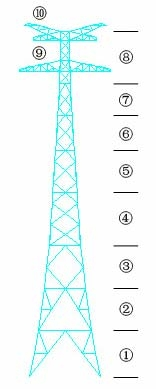
\includegraphics[width=0.3\textwidth]{tower_zone.jpg}
\caption{输电塔分层示意图}\label{fig:tower-zone}
\end{figure}

\begin{figure}[!htbp]
\centering
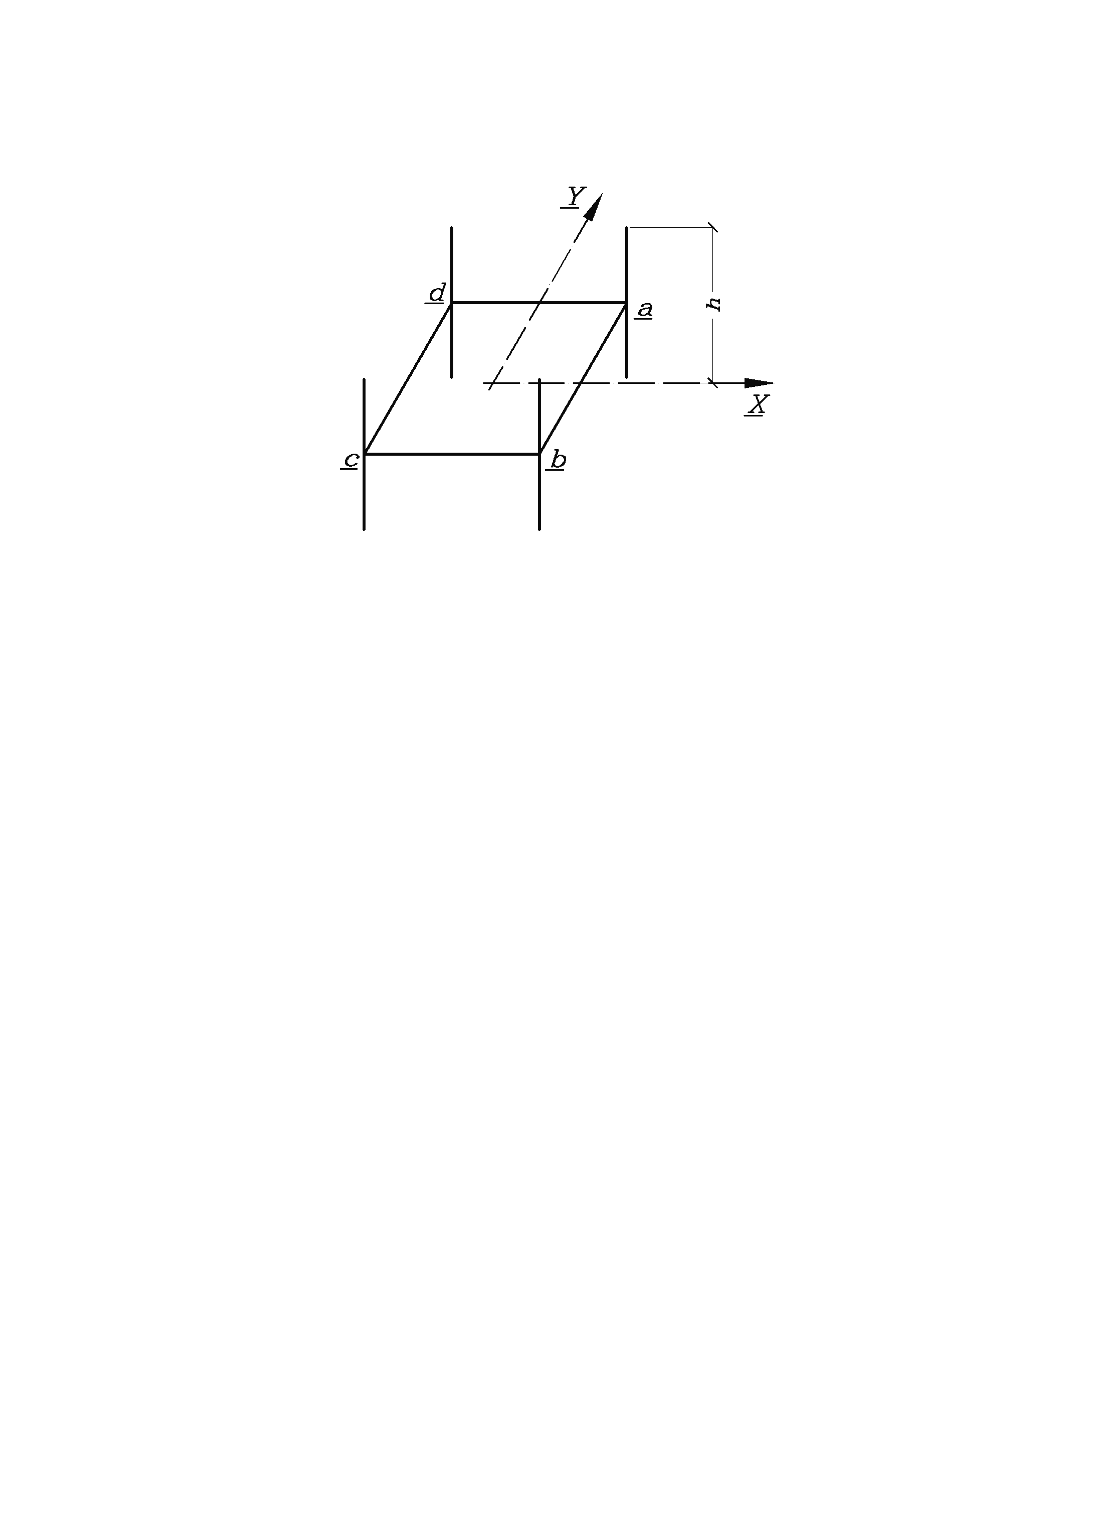
\includegraphics[width=0.6\textwidth]{tower_zone_diagram.pdf}
\caption{输电塔典型层示意图}\label{fig:tower-zone-diagram}
\end{figure}

\begin{enumerate}
\item 根据第\ref{sec:tornado}节计算输电塔节点a,b,c和d处龙卷风速度分量 $V_x$和$V_y$;
\item 分别沿$X$和$Y$方向计算风速风量的均值$V_x'$和$V_y'$;
\item 计算输电塔节点a,b,c和d处所在层龙卷风荷载,值得注意的是公式中各物理量采用SI单位制,即风速单位为\SI{}{m/s},风荷载单位为\SI{}{N}。

根据美国ASCE规范,该层$X$和$Y$方向龙卷风荷载$F_{\mathrm{w}x}$和$F_{\mathrm{w}y}$为
\begin{equation}
F_{\mathrm{w}x} = 0.613 (V_{x}')^2 C_{\mathrm{f}x} A_x
\end{equation}
\begin{equation}
F_{\mathrm{w}y} = 0.613 (V_{y}')^2 C_{\mathrm{f}y} A_y
\end{equation}
其中,$A_x$和$A_y$分别为该层迎风面构件沿$X$和$Y$方向的投影面积。
风压系数由\ref{fig:force-coefficient}计算。

根据中国规范,该层$X$和$Y$方向龙卷风荷载$F_{\mathrm{w}x}$和$F_{\mathrm{w}y}$为
\begin{equation}
F_{\mathrm{w}x} = 0.625 (V_{x}')^2 \mu_{\mathrm{s}x} A_x 
\end{equation}
\begin{equation}
F_{\mathrm{w}y} = 0.625 (V_{y}')^2 \mu_{\mathrm{s}y} A_y 
\end{equation}
体型系数$\mu_\mathrm{s} = 1.3(1+\eta)$,$\eta$由表\ref{tab:eta}计算。

可知中美规范计算龙卷风荷载的公式的主要区别如下:中国将风速转化为速度压的系数为$\SI{0.625}{kg/m^3}$,美国为$1/2\rho_a=\SI{0.613}{kg/m^3}$,中国规范稍微偏保守;二者的主要差别为体型系数(风压系数)的计算:对于圆形截面输电塔,$\Phi<0.025$的层,美国规范的风压系数为$C_\mathrm{f}=4.0\times0.67=2.68$,中国规范为$\mu_\mathrm{s}=1.3(1+\eta)=1.3 \times(1+1.0)=2.6$,相差不大,美国规范偏保守。

\item 迎风面和背风面上风荷载分配

中国规范根据塔架背风面荷载降低系数$\eta$对某层输电塔所受风荷载进行分配,即迎风面节点在$X$和$Y$方向所受风荷载分量分别为 $1/(1+\eta) F_{\mathrm{w}x}$ 和 $1/(1+\eta) F_{\mathrm{w}y}$;背风面节点在$X$和$Y$方向所受风荷载分量分别为 $\eta/(1+\eta) F_{\mathrm{w}x}$ 和 $\eta/(1+\eta) F_{\mathrm{w}y}$;

\item 迎(背)风面节点间风荷载分配

迎(背)风面上的节点根据各节点的投影面积进行迎(背)风面上风荷载的分配。


\end{enumerate}


\section{索的悬链线理论及输电线作用于塔的荷载}

\subsection{索的悬链线理论基本假设}
索由高强钢丝集束而成,相对抗弯刚度很小,其受力特点可以认为是完全柔性。
在自重和张力作用下分析其线形和力学参数时,基本假设如下:
\begin{itemize}
\item
索是理想柔性,既不能受压也不能受弯;
\item
索的材料符合胡克定律;
\item
索的横截面积在外荷载作用下的变化量十分微小,可忽略不计。
\end{itemize}

为了确定重力作用下索的线形,以弦左端点为原点、竖直向上为Y轴正方向建立右手直角坐标系。
则索受到的重力沿Y轴负向。
假设单位长度索的质量恒定,且不随张力变化。

\begin{figure}[!htbp]
  \centering
  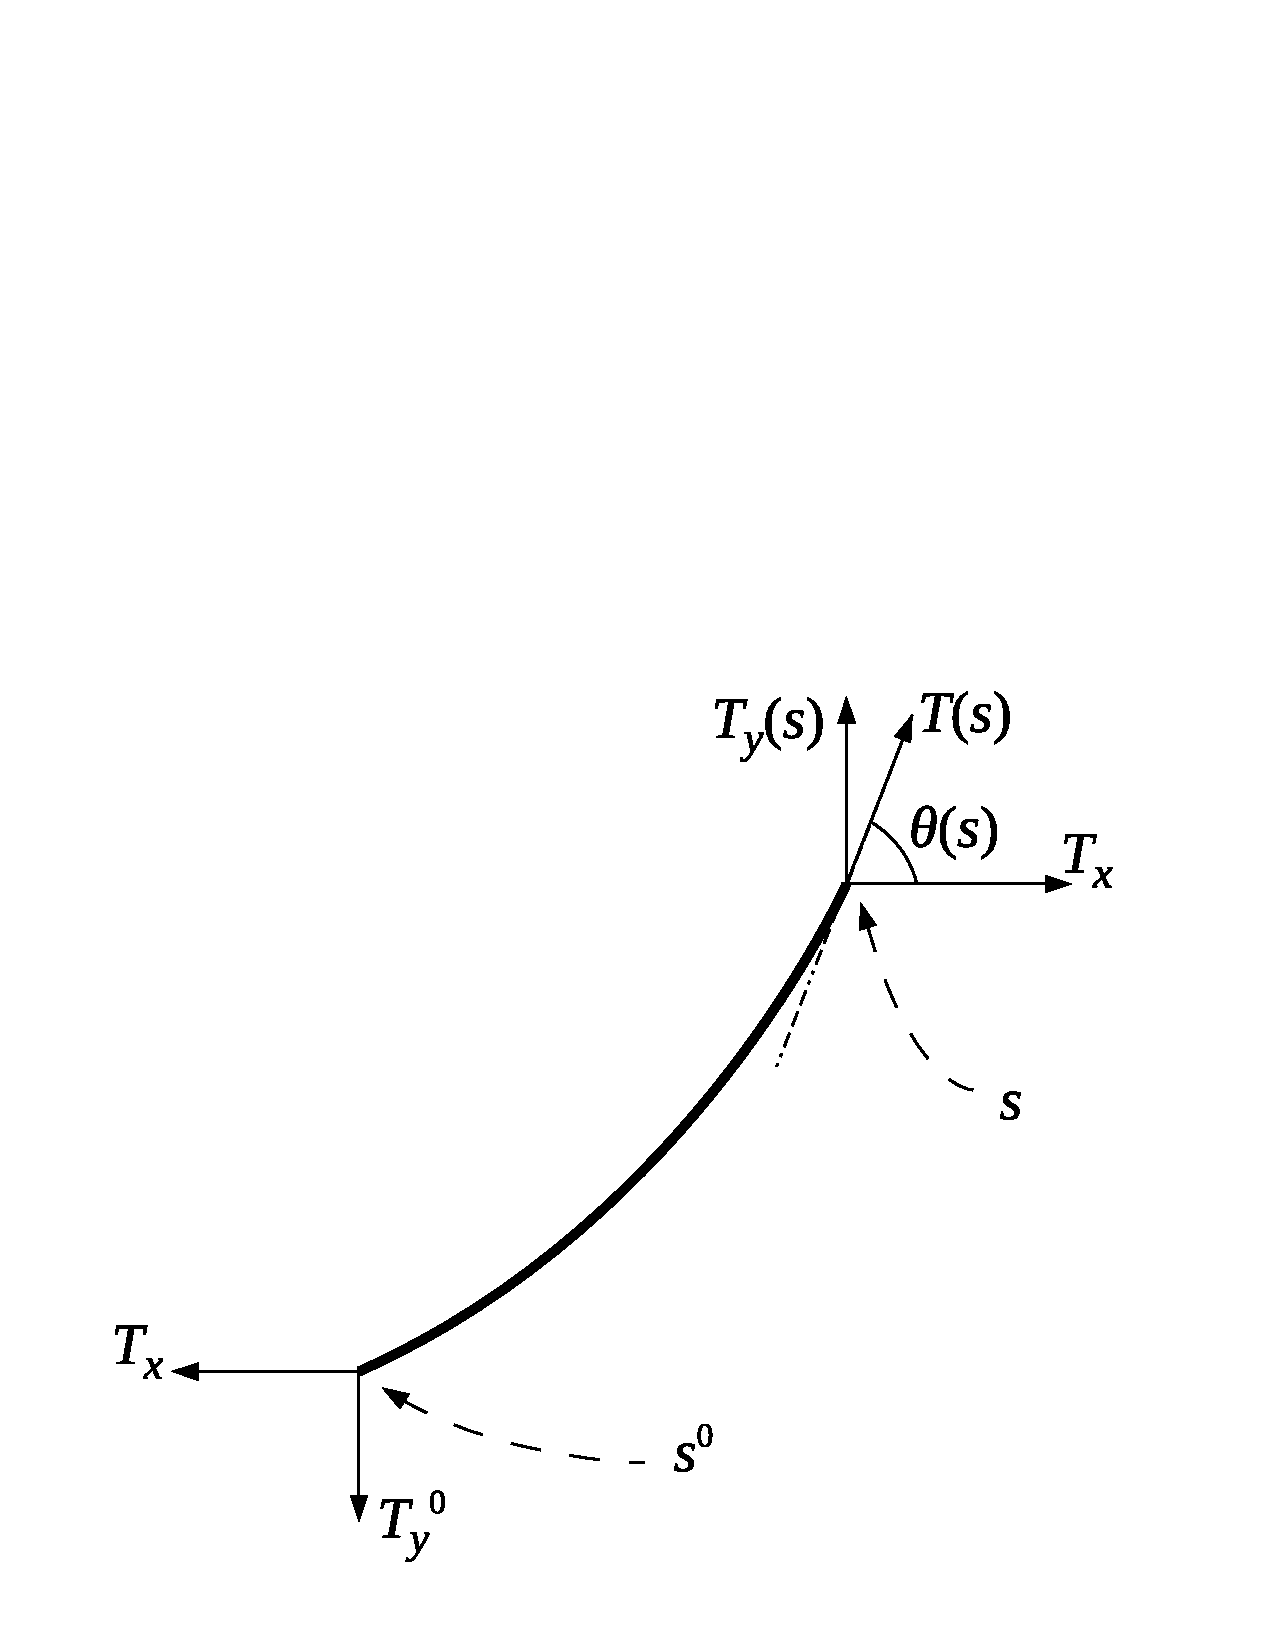
\includegraphics[width=0.6\textwidth]{catenary_diagram.pdf}
  \label{fig:catenary}
  \caption{索段计算示意图}
\end{figure}

\subsection{符号约定}
\begin{description}
  \item[$s$]
  从索左端点(坐标系原点)开始计算的索长度;
  \item[$\mu$]
  单位长度索的质量(假设是恒定的);
  \item[$T(s)$]
  索长度为$s$处的索张力(根据柔性索假设,张力沿索的切线方向);
  \item[$T_y(s)$]
  索长度为$s$处的索张力的$Y$向分量;
  \item[$T_x$]
  张力的$X$向分量(任取索段进行受力分析,由$X$向平衡方程可知$T_x$沿索长是均匀的);
  \item[$\theta(s)$]
  索切向量与$X$轴正向的夹角。
\end{description}

\subsection{自重作用下的单索线形求解}
索段竖向的平衡方程为:
\begin{gather}
  T_y(s) = g \int_{s^0}^{s} \mu \mathrm{d}s + T_y^0 \notag \\
  T_x \tan(\theta(s)) = g \mu \int_{s^0}^{s} \mathrm{d}s + T_y^0 \notag \\
  T_x \frac{\mathrm{d} y}{\mathrm{d} x} = g \mu \int_{s^0}^{s} \sqrt{1+\left(\frac{\mathrm{d} y}{\mathrm{d} x}\right)^2} \mathrm{d}x + T_y^0 \notag \\
  \frac{\mathrm{d}^2 y}{\mathrm{d} x^2} = \frac{g \mu}{T_x} \sqrt{1+\left(\frac{\mathrm{d} y}{\mathrm{d} x}\right)^2}
\end{gather}
此二阶微分方程的解析解为:
\begin{equation}
  y = \frac{T_x}{g \mu} \cosh \left( \frac{g \mu}{T_x} + c_1 \right)+c_2
\end{equation}
式中,$c_1$和$c_2$为由边界条件确定的积分常量。代入边界条件:$x=0,y=0;x=L,y=C$(见图\ref{fig:cat})。

\begin{figure}[!htpb]
\centering
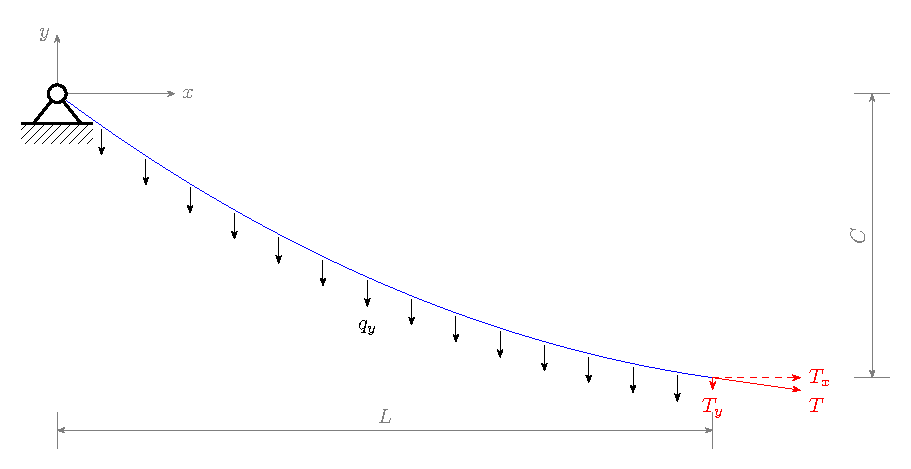
\includegraphics[width=0.8\textwidth]{cat.pdf}
\caption{单缆尺寸及边界条件示意图}
\label{fig:cat}
\end{figure}

\begin{equation}
  \left \{
    \begin{split}
      & \beta = \frac{g \mu L}{2 T_x}\\
      & c_1 = \sinh^{-1}\left(\frac{\beta C / L}{\sinh \beta}\right)\\
      & c_2 = -\frac{T_x}{g \mu} \cosh(c_1)
    \end{split}
  \right.
\end{equation}

悬链线索的形状长度$S$和无应力长度$S_0$分别为:
\begin{equation}
  S = \frac{T_x}{g\mu}\left[\sinh\left(\frac{g \mu L}{T_x}+c_1\right)+\sinh(c_1)\right]
\end{equation}

\begin{equation}
\begin{split}
  S_0 &= S-\Delta S \\
      &= S - \frac{T_x}{EA g \mu }\left[ \frac{1}{2} g \mu L + \frac{1}{8} T_x \left( e^{2(c_1+2\beta)} - e^{-2(c_1-2\beta)} -e^{2c_1} + e^{-2c_1} \right) \right]
\end{split}
\end{equation}

\subsection{输电线施加在输电塔的荷载求解}

跨越塔之间输电线跨度为$L=\SI{1770}{m}$,右侧支座比左侧支座高度相同,即$C=\SI{0}{}$,跨中矢高$f=\SI{132.4}{m}$,单位长度质量$\mu=\SI{3219}{kg/km}$。
索的弹性模量$E=\SI{108070}{MPa}$,截面积$A=\SI{729}{mm^2}$。
假设在外荷载作用下两支座的间距及高差保持不变。
主要任务是利用上述悬链线理论计算输电线对输电塔施加的荷载。

主要思路:输电线在自重和张力作用下,其线形为悬链线,故可采用悬链线经典公式来进行求解。
采用直接建模的方式,单缆采用LINK1单元模拟,单元水平长度为\SI{1}{m}。
分析时,首先假定水平力大小,根据悬链线方程求解节点坐标,由此建立节点和单元,并分析单缆在自重作用下的内力和线形。
如果求解获得的水平力与假定水平力之间的误差较大或者单缆变形较大,则返回重新计算,直至满足误差要求。计算框图如图\ref{fig:flow-chart}所示。
\begin{figure}[!htpb]
\centering
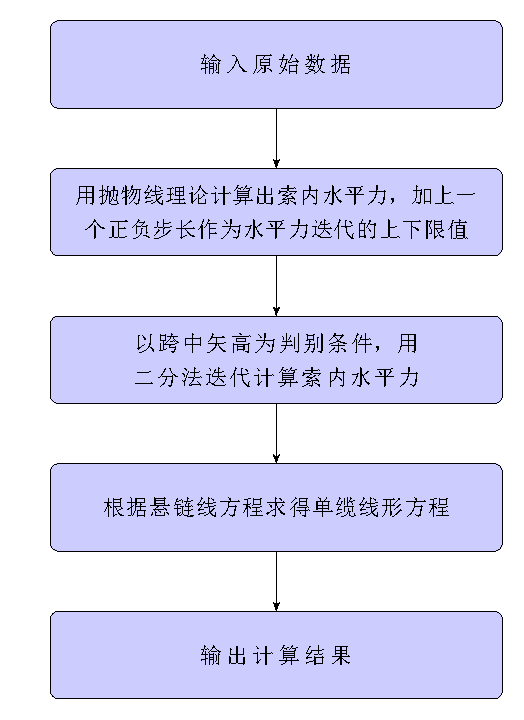
\includegraphics[width=0.4\textwidth]{flow_chart.pdf}
\caption{单缆线形和力学参数计算框图}
\label{fig:flow-chart}
\end{figure}

计算的APDL和MATLAB程序见附录\ref{apen:cat}。如图\ref{fig:cat-disp}所示,\SI{12.7}{mm},相比于跨径$L=\SI{1770}{m}$该变形已足够小,认为已满足精度要求。

\begin{figure}[!htbp]
\centering
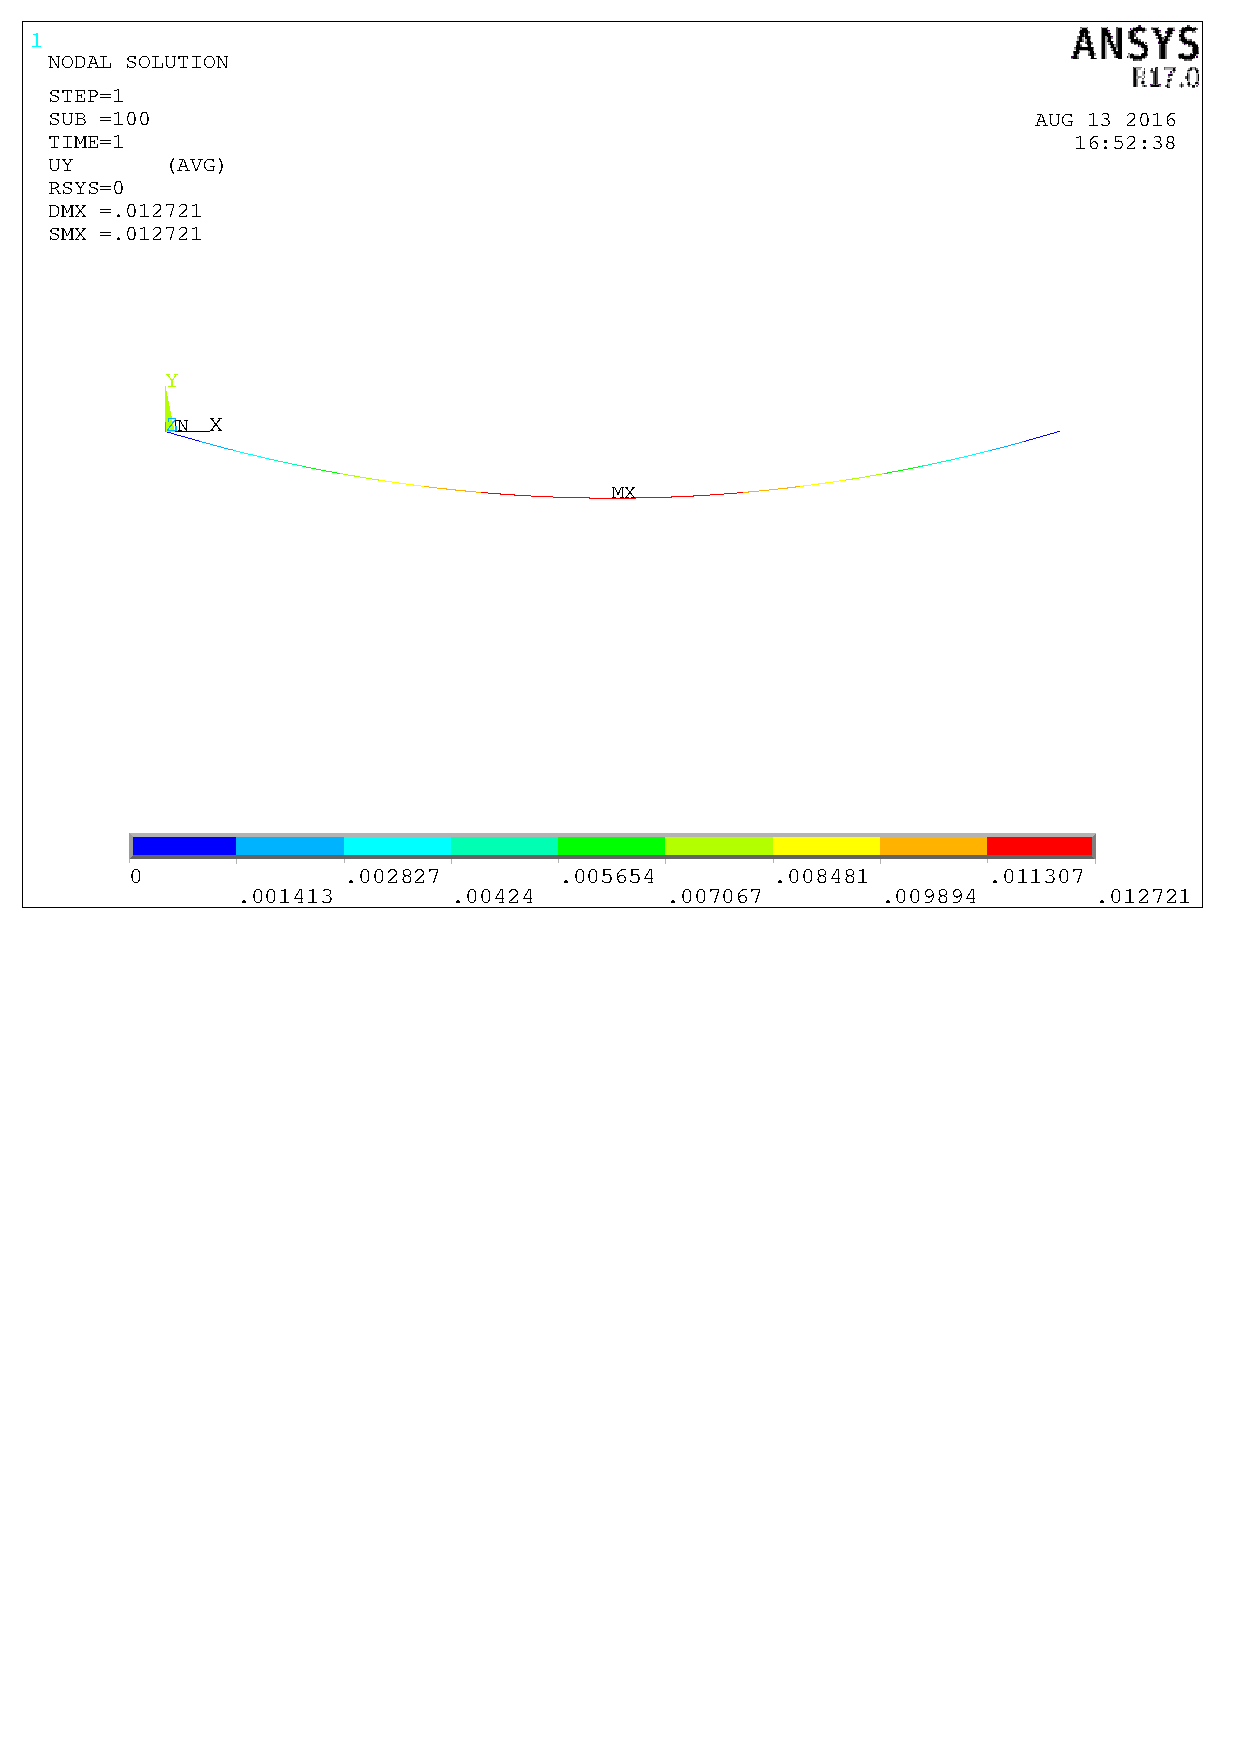
\includegraphics[width=0.8\textwidth]{cat_disp.pdf}
\caption{跨越塔之间输电线变形图(单位:\SI{}{m})}
\label{fig:cat-disp}
\end{figure}

对于跨越塔和锚塔之间的输电线对跨越塔的荷载计算采用相同的方法,在此不一一列举。

跨越塔受到的两侧输电线传来的张力的示意图见图\ref{fig:line-force}所示。

\begin{figure}[!htbp]
\centering
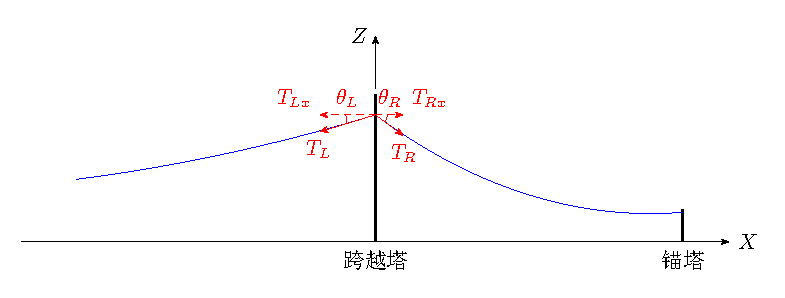
\includegraphics[width=0.8\textwidth]{line_force}
\caption{跨越塔受到输电线的张力示意图}
\label{fig:line-force}
\end{figure}

经过附录\ref{apen:cat}程序的计算,图\ref{fig:line-force}中各量为:
\begin{equation}
\begin{split}
  T_{Lx} & = \SI{93.31}{kN},\quad \theta_L  = \ang{16.89} \\
  T_{Rx} & = \SI{21.33}{kN},\quad \theta_L  = \ang{36.70}
\end{split}
\end{equation}



\section{龙卷风位置变化的参数分析}
\subsection{位移响应参数化分析}
利用附录\ref{apen:static}中的APDL程序进行龙卷风作用下输电塔结构的静力响应分析,
并改变龙卷风核心位置$(R, \theta)$(见图\ref{fig:tower-tornado-cs}),
分析其对输电塔塔顶位移响应的影响,如表\ref{tab:disp}和图\ref{fig:disp}所示。

\begin{table}[!htbp]
  \centering
  \caption{塔顶位移响应(\SI{}{mm})随龙卷风核心位置的参数化分析}
  \label{tab:disp}
  \begin{tabu} to 1.0\textwidth {X[1.5,c] X[1,r] X[1,r] X[1,r] X[1,r] X[1,r] X[1,r] X[1,r]}
    \toprule
    \diagbox{$R/\SI{}{m}$}{$\theta/\SI{}{\degree}$} & 0 & 15 & 30 & 45 & 60 & 75 & 90 \\
    \midrule
    500 &  377.3 & 434.4 &  537.1 &  607.8 &  430.5 &  459.3 &  367.5 \\
    450 &  425.1 & 475.6 &  601.5 &  674.6 &  465.9 &  509.5 &  411.1 \\
    400 &  479.1 & 517.4 &  675.1 &  743.4 &  502.6 &  563.2 &  459.9 \\
    350 &  542.6 & 560.2 &  763.1 &  814.3 &  542.5 &  621.6 &  517.9 \\
    300 &  629.4 & 611.6 &  886.2 &  898.1 &  596.7 &  694.5 &  602.1 \\
    250 &  775.4 & 699.7 & 1092.5 & 1027.3 &  700.6 &  811.8 &  755.6 \\
    200 & 1001.8 & 842.8 & 1403.9 & 1199.9 &  885.5 &  984.1 & 1010.8 \\
    150 & 1139.5 & 920.6 & 1567.2 & 1232.6 & 1016.9 & 1063.0 & 1175.6 \\
    120 & 1042.8 & 823.9 & 1394.7 & 1035.9 &  942.6 &  952.0 & 1059.3 \\
    100 &  794.7 & 626.0 & 1105.3 &  756.2 &  736.0 &  710.3 &  843.8 \\
    \bottomrule
  \end{tabu}
\end{table}
可知,塔顶位移响应的危险工况位于$\theta=\SI{30}{\degree}$附近,
且径向位置靠近核心半径$r_c=\SI{120}{m}$处。

\begin{figure}[!htbp]
  \centering
  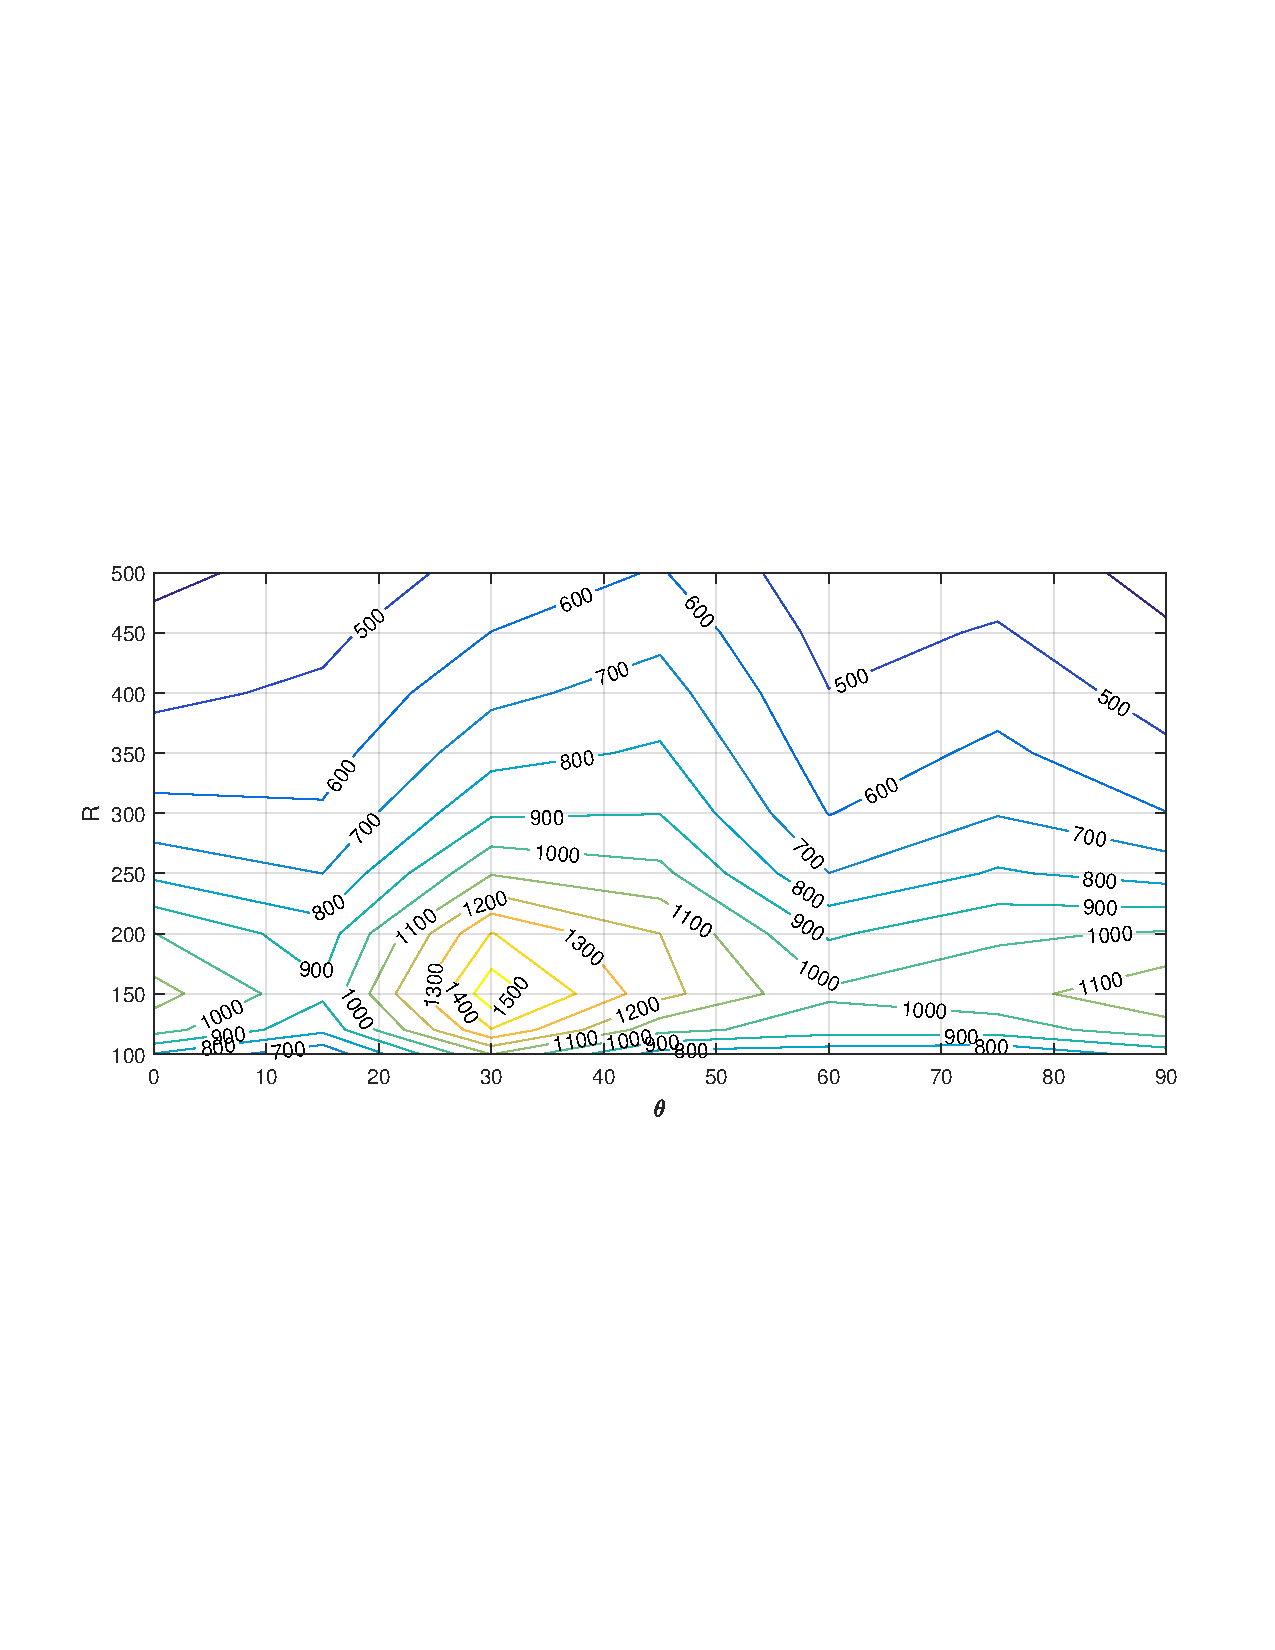
\includegraphics[width=1.0\textwidth]{disp.pdf}
  \caption{输电塔位移响应随龙卷风核心位置变化的等值线图}
  \label{fig:disp}
\end{figure}



\end{document}
